%!TeX root = book.tex
%!TEX TS-program = lualatex

\begin{russian}
\chapter[Механика упругого деформирования пространства с периодической системой полостей или включений]{Механика упругого деформирования пространства с~периодической системой полостей или включений}\chaptermark{Пространство с периодической системой полостей или включений}

\section[Упругое пространство с периодической системой сферических полостей]{Упругое пространство с периодической системой сферических полостей\sectionmark{Упругое пространство с периодической системой сферических полостей}}\sectionmark{Упругое пространство с периодической системой сферических полостей}

Рассмотрим упругое пространство $\Omega$ и бесконечную систему сферических полостей $\{\omega_{\alpha\beta\gamma}\}_{\alpha,\beta,\gamma=-\infty}^\infty$, центры которых расположены в узлах $\{O_{\alpha\beta\gamma}\}_{\alpha,\beta,\gamma=-\infty}^\infty$ кубической периодической решетки со стороной $a$. Декартовыми координатами узлов решетки будут упорядоченные наборы чисел $\{(\alpha a,\beta a,\gamma a);\,\alpha,\beta,\gamma\in\mathbb{Z}\}$. Радиусы полостей обозначим через $R$. Применим линейное упорядочение к узлам решетки, перенумеровав их согласно правилу\sloppy
$$
n(O_{\alpha_1,\beta_1,\gamma_1})>n(O_{\alpha_2,\beta_2,\gamma_2}),
$$
если 
\begin{multline}
\bigg\{|\alpha_1|+|\beta_1|+|\gamma_1|>|\alpha_2|+|\beta_2|+|\gamma_2|\bigg\}\bigvee \\
\bigvee\bigg\{\Big(|\alpha_1|+|\beta_1|+|\gamma_1|=|\alpha_2|+|\beta_2|+|\gamma_2|\Big)\bigwedge\Big((\alpha_1>\alpha_2)\bigvee \\
\bigvee(\alpha_1=\alpha_2,\beta_1>\beta_2)\bigvee(\alpha_1=\alpha_2,\beta_1=\beta_2,\gamma_1>\gamma_2)\Big)\bigg\}.
\end{multline}

\begin{figure}[h!]
\centering
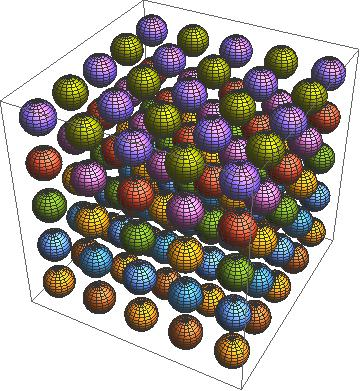
\includegraphics[width=7cm]{cav-125.jpg}
\caption{Периодическая система сферических полостей в упругом пространстве}
\label{f:11:1f}
\end{figure}

Выше обозначен через $n(O_{\alpha_1,\beta_1,\gamma_1})$ номер узла $O_{\alpha_1,\beta_1,\gamma_1}$. В новой нумерации точка $O_{\alpha,\beta,\gamma}$ обозначается через $O_j$ (рис.~\ref{f:11:1}).

\begin{figure}[h!]
\centering
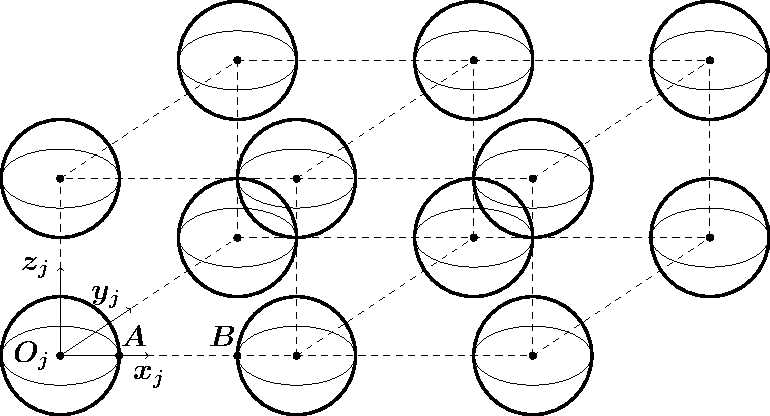
\includegraphics[width=12cm]{cartesian-spheres-periodic.pdf}
\caption{Схематическое представление задачи}
\label{f:11:1}
\end{figure}

С каждой точкой $O_j$ свяжем локальные декартовую $(x_j,y_j,z_j)$ и сонаправленную с ней сферическую системы координат $(r_j,\theta_j,\varphi_j)$. Считается, что декартовые системы координат с началами в точках $O_j$ сонаправлены.

Будем рассматривать задачу упругого деформирования пространства со сферическими полостями $\Omega\backslash\bigg\{\bigcup\limits_{\alpha,\beta,\gamma}\omega_{\alpha\beta\gamma}\bigg\}$ под действием нагрузки, приложенной на бесконечности (одноосное, двуосное или всестороннее растяжение упругого пространства). Сферические полости считаются свободными от нагрузки.

Соотношения между координатами можно описать формулами

\begin{equation*}
{x_i} = {r_i}\sin {\theta _i}\cos {\varphi _i},
\end{equation*}

\begin{equation}
{y_i} = {r_i}\sin {\theta _i}\sin {\varphi _i},
\label{eq:11:1}
\end{equation}

\begin{equation*}
{z_i} = {r_i}\cos {\theta _i},
\end{equation*}

\begin{equation}
\left\{ {\begin{array}{*{20}{l}}
{{x_j} = {x_\alpha } + {x_{j\alpha }},}\\
{{y_j} = {y_\alpha } + {y_{j\alpha }},}\\
{{z_j} = {z_\alpha } + {z_{j\alpha }},}
\end{array}} \right.\qquad {\kern 1pt} j \ne \alpha ,\quad j,\alpha  = \overline {1,N},
\label{eq:11:2}
\end{equation}

\noindent где $\overrightarrow {{O_j}{O_\alpha }}  = \left( {{x_{j\alpha }},{y_{j\alpha }},{z_{j\alpha }}} \right) = \left( {{r_{j\alpha }},{\theta _{j\alpha }},{\varphi _{j\alpha }}} \right)$.

Для определения НДС в рассматриваемом теле необходимо решить краевую задачу для уравнения Ламе относительно неизвестного вектора перемещения   $\mathbf{U}$ с граничными условиями

\begin{equation}
{\bf{FU}}{|_{{\Gamma _j}}} = 0
\end{equation}

\noindent и условиями на бесконечности одного из трех типов

\begin{equation}
{\bf{FU}}{|_{z =  \pm \infty }} =  \pm T{{\bf{e}}_z}\quad\text{(одноосное растяжение)},
\label{eq:11:1a}
\end{equation}

\begin{equation}
{\bf{FU}}{|_{\rho  = \infty }} = T{{\bf{e}}_\rho }\quad\text{(двуосное растяжение)},
\label{eq:11:2a}
\end{equation}

\begin{equation}
{\bf{FU}}{|_{r  = \infty }} = T{{\bf{e}}_r }\quad\text{(всестороннее растяжение)},
\label{eq:11:3a}
\end{equation}

\noindent где $\mathbf{FU}$~--- отвечающий перемещению $\mathbf{U}$ вектор усилий на соответствующей граничной поверхности, ${\Gamma _j} = \left\{ {\left( {{r_j},{\theta _j},{\varphi _j}} \right):\,{r_j} = {R_j}} \right\}$.

Решение задачи будем искать в виде

\begin{equation}
{\bf{U}} = {\bf{\tilde U}} + {{\bf{U}}_0},
\label{eq:11:8s}
\end{equation}

\begin{equation}
{\bf{\tilde U}} = \sum\limits_{j = 1}^\infty {\sum\limits_{s = 1}^3 {\sum\limits_{n = 0}^\infty  {\sum\limits_{m=-n}^{n} {a_{s,n,m}^{(j)}} } } } {\bf{\tilde U}}_{s,n,m}^{ + (4)}\left( {{r_j},{\theta _j},{\varphi _j}} \right),
\label{eq:11:8a}
\end{equation}

\begin{equation}
{{\bf{U}}_0} = \frac{T}{{2G}}\left( { - \frac{\sigma }{{1 + \sigma }}{\rho}{{\bf{e}}_{{\rho}}} + \frac{1}{{1 + \sigma }}{z}{{\bf{e}}_z}} \right)\,\text{(одноосное растяжение)},
\label{eq:11:8}
\end{equation}

\begin{equation}
{{\bf{U}}_0} = \frac{T}{{2G}}\left( {\frac{{1 - \sigma }}{{1 + \sigma }}{\rho}{{\bf{e}}_{{\rho}}} - \frac{{2\sigma }}{{1 + \sigma }}{z}{{\bf{e}}_z}} \right)\,\text{(двуосное растяжение)},
\label{eq:11:9}
\end{equation}

\begin{equation}
{{\bf{U}}_0} = \frac{T}{2G}\frac{1-2\sigma}{1+\sigma}\left(\rho\mathbf{e}_\rho+z\mathbf{e}_z\right)\,\text{(всестороннее растяжение)},
\label{eq:11:9a}
\end{equation}

\noindent где $G$, $\sigma$~--- модуль сдвига и коэффициент Пуассона упругого пространства; $a_{s,n,m}^{(j)}$~--- неизвестные коэффициенты; перемещения $\mathbf{\tilde U}_{s,n,m}^{+(4)}$ приведены в формулах~\eqref{eq:1:89b}~--- \eqref{eq:1:94b}.

Относительно перемещения $\mathbf{\tilde U}$ граничные условия записываем следующим образом:

\begin{equation}
{\bf{F\tilde U}}{|_{{\Gamma _j}}} =  - {\bf{F}}{{\bf{U}}_0}{|_{{\Gamma _j}}};
\label{eq:11:5}
\end{equation}

\begin{equation}
{\bf{F\tilde U}}{|_{z =  \pm \infty }} = 0\quad\text{(одноосное растяжение)},
\label{eq:11:3}
\end{equation}

\begin{equation}
{\bf{F\tilde U}}{|_{\rho  = \infty }} = 0\quad\text{(двуосное растяжение)},
\label{eq:11:4}
\end{equation}

\begin{equation}
{\bf{F\tilde U}}{|_{r  = \infty }} = 0\quad\text{(всестороннее растяжение)}.
\label{eq:11:4a}
\end{equation}

Вспомогательным перемещениям $\mathbf{U}_0$ отвечают следующие напряжения на поверхностях $\Gamma_j$ ($\mathbf{n}_j=\mathbf{e}_{r_j}$~--- вектор нормали на поверхности $\Gamma_j$):

\begin{equation}
{\bf{F}}{{\bf{U}}_0} = T{P_1}(\cos {\theta _j}){{\bf{e}}_z}\quad\text{(одноосное растяжение)},
\end{equation}

\begin{equation}
{\bf{F}}{{\bf{U}}_0} =  - TP_1^{(1)}(\cos {\theta _j}){{\bf{e}}_{{\rho _j}}}\quad\text{(двуосное растяжение)},
\end{equation}

\begin{multline}
\mathbf{FU}_0=T\bigg[-P_1^{(1)}(\cos\theta_j)\mathbf{e}_{\rho_j}+ \\
+P_1(\cos\theta_j)\mathbf{e}_z\bigg]\,\text{(всестороннее растяжение)}.
\end{multline}

Используя теоремы сложения~\eqref{eq:1:99t}, перемещение $\mathbf{\tilde U}$ можно записать полностью в системе координат с началом в точке $O_j$:

\begin{multline}
{\bf{\tilde U}} = \sum\limits_{s = 1}^3 {\sum\limits_{n = 0}^\infty  {\sum\limits_{m =  - n }^{n } {a_{s,n,m}^{(j)}} } } {\bf{\tilde U}}_{s,n,m}^{ +(4)}\left( {{r_j},{\theta _j},{\varphi _j}} \right) + \\
+ \sum\limits_{s=1}^3\sum\limits_{n = 0}^\infty\sum\limits_{m =  - n }^{n }{\bf{\tilde U}}_{s,n,m}^{ - (4)}\left( {{r_j},{\theta _j},{\varphi _j}} \right)\sum\limits_{\alpha  \ne j}\sum\limits_{t=1}^3\sum\limits_{k = 0}^\infty\mathop \sum \limits_{l =  - k}^{k}\tilde T_{t,k,l,\alpha}^{s,n,m,j}a_{t,k,l}^{(\alpha)}.
\label{eq:11:10}
\end{multline}

%Формулы для напряжений, отвечающих базисным функциям перемещений $\mathbf{U}_{s,n,m}^{\pm(4)}(r_j,\theta_j,\varphi_j)$ на сферических поверхностях $\Gamma_j$ ($\mathbf{n}_j=\mathbf{e}_{\rho_j}$, $\mathbf{n}_j$~--- нормаль к поверхности $\Gamma_j$):
%
%\begin{multline}
%{\bf{FU}}_{1,n,m}^{ + (4)}\left( {{r_j},{\theta _j},{\varphi _j}} \right) =  - \frac{{2G}}{{{r_j}}}(n + 1)\left[ { - u_{n,m - 1}^{ + (4)}\left( {{r_j},{\theta _j},{\varphi _j}} \right){{\bf{e}}_{ - 1}} + } \right.\\
%\left. { + u_{n,m + 1}^{ + (4)}\left( {{r_j},{\theta _j},{\varphi _j}} \right){{\bf{e}}_1} - u_{n,m}^{ + (4)}\left( {{r_j},{\theta _j},{\varphi _j}} \right){{\bf{e}}_0}} \right],
%\end{multline}
%
%\begin{multline}
%{\bf{FU}}_{2,n,m}^{ + (4)}\left( {{r_j},{\theta _j},{\varphi _j}} \right) = \frac{{2G}}{{{r_j}}}\left\{ {(n + m)\left[ {\frac{{(n + 3)(n - m + 2)}}{{2n + 3}} - 2\sigma } \right] \times } \right.\\
%\times u_{n,m - 1}^{ + (4)}\left( {{r_j},{\theta _j},{\varphi _j}} \right){{\bf{e}}_{ - 1}} - \\
%- (n - m)\left[ {\frac{{(n + 3)(n + m + 2)}}{{2n + 3}} - 2\sigma } \right]u_{n,m + 1}^{ + (4)}\left( {{r_j},{\theta _j},{\varphi _j}} \right){{\bf{e}}_1} + \\
%+ \left[ {\frac{{(n + 3)(n - m + 1)(n + m + 1)}}{{2n + 3}} - (n + 1)(2\sigma  - 1)} \right] \times \\
%\times u_{n,m}^{ + (4)}\left( {{r_j},{\theta _j},{\varphi _j}} \right){{\bf{e}}_0} \bigg\},
%\end{multline}
%
%\begin{multline}
%{\bf{FU}}_{3,n,m}^{ + (4)}\left( {{r_j},{\theta _j},{\varphi _j}} \right) =  - \frac{{2G}}{{{r_j}}}\left[ {(n - m + 2)u_{n,m - 1}^{ + (4)}\left( {{r_j},{\theta _j},{\varphi _j}} \right){{\bf{e}}_{ - 1}} + } \right.\\
%\left. { + (n + m + 2)u_{n,m + 1}^{ + (4)}\left( {{r_j},{\theta _j},{\varphi _j}} \right){{\bf{e}}_1} - mu_{n,m}^{ + (4)}\left( {{r_j},{\theta _j},{\varphi _j}} \right){{\bf{e}}_0}} \right],
%\end{multline}
%
%\begin{multline}
%{\bf{FU}}_{1,n,m}^{ - (4)}\left( {{r_j},{\theta _j},{\varphi _j}} \right) = \frac{{2G}}{{{r_j}}}n\bigg[ - u_{n,m - 1}^{ - (4)}\left( {{r_j},{\theta _j},{\varphi _j}} \right){{\bf{e}}_{ - 1}} + \\
%+ u_{n,m + 1}^{ - (4)}\left( {{r_j},{\theta _j},{\varphi _j}} \right){{\bf{e}}_1} + u_{n,m}^{ - (4)}\left( {{r_j},{\theta _j},{\varphi _j}} \right){{\bf{e}}_0} \bigg],
%\end{multline}
%
%\begin{multline}
%{\bf{FU}}_{2,n,m}^{ - (4)}\left( {{r_j},{\theta _j},{\varphi _j}} \right) = \\
%= \frac{{2G}}{{{r_j}}}\left\{ { - (n - m + 1)\left[ {\frac{{(n - 2)(n + m - 1)}}{{2n - 1}} + 2\sigma } \right] \times } \right.\\
%\times u_{n,m - 1}^{ - (4)}\left( {{r_j},{\theta _j},{\varphi _j}} \right){{\bf{e}}_{ - 1}} + (n + m + 1)\left[ {\frac{{(n - 2)(n - m - 1)}}{{2n - 1}} + 2\sigma } \right] \times \\
%\times u_{n,m + 1}^{ + (4)}\left( {{r_j},{\theta _j},{\varphi _j}} \right){{\bf{e}}_1} + \\
%\left. { + \left[ {\frac{{(n - 2)(n - m)(n + m)}}{{2n - 1}} + n(2\sigma  - 1)} \right]u_{n,m}^{ - (4)}\left( {{r_j},{\theta _j},{\varphi _j}} \right){{\bf{e}}_0}} \right\},
%\end{multline}
%
%\begin{multline}
%{\bf{FU}}_{3,n,m}^{ - (4)}\left( {{r_j},{\theta _j},{\varphi _j}} \right) = \frac{{2G}}{{{r_j}}}\left[ {(n + m - 1)u_{n,m - 1}^{ - (4)}\left( {{r_j},{\theta _j},{\varphi _j}} \right){{\bf{e}}_{ - 1}} + } \right.\\
%\left. { + (n - m - 1)u_{n,m + 1}^{ - (4)}\left( {{r_j},{\theta _j},{\varphi _j}} \right){{\bf{e}}_1} - mu_{n,m}^{ - (4)}\left( {{r_j},{\theta _j},{\varphi _j}} \right){{\bf{e}}_0}} \right].
%\end{multline}

В силу периодичности задачи вклад каждого слагаемого в формуле~\eqref{eq:11:8a} будет одинаковым, поэтому можно считать, что $a_{s,n,m}^{(j)}=a_{s,n,m}$.

После перехода в формуле~\eqref{eq:11:10} к напряжениям и удовлетворения граничным условиям относительно неизвестных $a_{s,n,m}$ получаем бесконечную систему линейных алгебраических уравнений:

\begin{equation}
\sum\limits_{s=1}^3 a_{s,n,m}\tilde F_{s,n,m}^{+(k)}+\tilde F_{s,n,m}^{-(k)}\sum\limits_{t=1}^3\sum\limits_{k=0}^\infty\sum\limits_{l=-k}^k a_{t,k,l}\sum\limits_{\alpha\neq j}\tilde T_{t,k,l,\alpha}^{s,n,m,j}=F_{n,m}^{(k)};
\label{eq:11:sys}
\end{equation}
$$
n,m \in\mathbb{Z}:\quad n \ge 0,{\mkern 1mu} \quad {\kern 1pt} |m| \le n,\quad {\mkern 1mu} k =  - 1,{\mkern 1mu} {\kern 1pt} 0,{\mkern 1mu} {\kern 1pt} 1;\;\;\;{\mkern 1mu} {\kern 1pt} j = \overline {1,\infty},
$$

\noindent где $\tilde F_{s,n,m}^{\pm(k)}$~--- компоненты вектора напряжений на поверхности $r_j=R$, отвечающего вектору перемещения $\tilde U_{s,n,m}^{\pm(4)}$:

$$
\mathbf{F\tilde U}_{s,n,m}^{\pm(4)}=\tilde F_{s,n,m}^{\pm(-1)}S_n^{m-1}\mathbf{e}_{-1}+\tilde F_{s,n,m}^{\pm(1)}S_n^{m+1}\mathbf{e}_1+\tilde F_{s,n,m}^{\pm(0)}S_n^m\mathbf{e}_0;
$$

\begin{equation*}
F_{n,m}^{(k)} =  -\frac{T}{2G}{\delta _{n1}}{\delta _{m0}}{\delta _{k0}}\quad\text{(одноосное растяжение)},
\label{eq:11:19}
\end{equation*}

\begin{equation*}
F_{n,m}^{(k)} =  -\frac{T}{2G}{\delta _{n1}}{\delta _{m0\,}}(2{\delta _{k, - 1}} - {\delta _{k1}})\quad\text{(двуосное растяжение)},
\label{eq:11:20}
\end{equation*}

\begin{equation*}
F_{n,m}^{(k)} =  -\frac{T}{2G}{\delta _{n1}}{\delta _{m0\,}}(\delta_{k0}+2{\delta _{k, - 1}} - {\delta _{k1}})\quad\text{(всестороннее растяжение)}.
\label{eq:11:21}
\end{equation*}

Явный вид компонент $\tilde F_{s,n,m}^{\pm(k)}$ не приводится ввиду их громоздкости. Они получаются из формул~\eqref{eq:1:89b}~--- \eqref{eq:1:99b}, \eqref{eq:8:f1}~--- \eqref{eq:8:f6}.

На рис.~\ref{f:11:4}~--- \ref{f:11:9} приведены нормальные напряжения на линии $AB$ в зависимости от расстояния между полостями при одноосном и двуосном растяжениях упругого пространства с периодической системой сферических полостей.

При одноосном растяжении основной вклад в тензор напряжений вносят напряжения $\sigma_z/T$. Областью их концентрации являются границы полостей. С приближением полостей друг к другу напряжения $\sigma_z/T$ возрастают.

При двуосном растяжении основной вклад в тензор напряжений вносят напряжения $\sigma_y/T$. Областью их концентрации являются границы полостей. С приближением полостей друг к другу напряжения $\sigma_y/T$ возрастают.

\begin{figure}[h!]
\centering\footnotesize
\parbox[b]{7.5cm}{\centering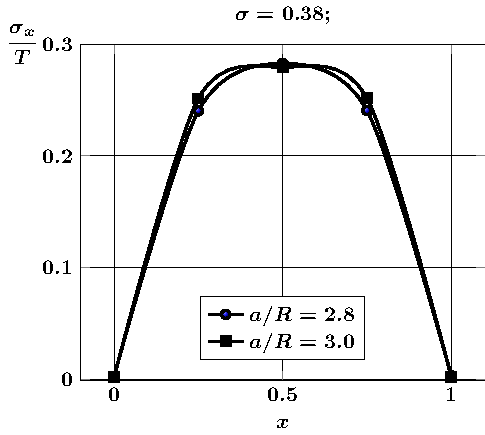
\includegraphics[width=7.6cm]{periodic-spheres-cav27-a-t1-sig_x.pdf}
\caption{Напряжения $\sigma_x/T$ на линии $AB$ в зависимости от расстояния между полостями при одноосном растяжении
\label{f:11:4}}}\hfil\hfil
\parbox[b]{7.5cm}{\centering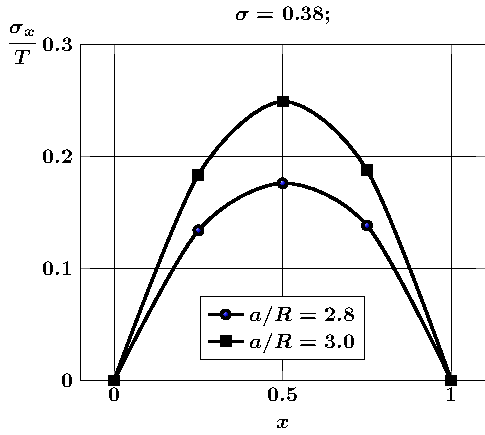
\includegraphics[width=7.6cm]{periodic-spheres-cav27-a-t2-sig_x.pdf}
\caption{Напряжения $\sigma_x/T$ на линии $AB$ в зависимости от расстояния между полостями при двуосном растяжении
\label{f:11:5}}}
\end{figure}

\begin{figure}[h!]
\centering\footnotesize
\parbox[b]{7.5cm}{\centering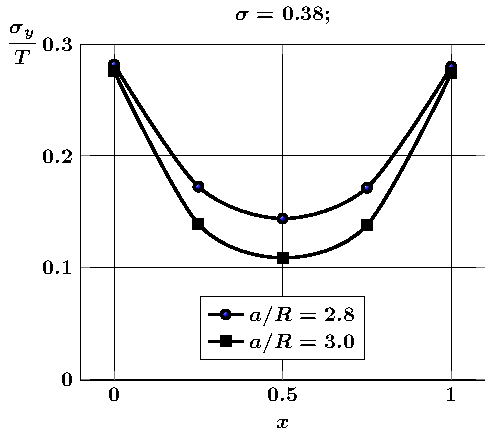
\includegraphics[width=7.6cm]{periodic-spheres-cav27-a-t1-sig_y.pdf}
\caption{Напряжения $\sigma_y/T$ на линии $AB$ в зависимости от расстояния между полостями при одноосном растяжении
\label{f:11:6}}}\hfil\hfil
\parbox[b]{7.5cm}{\centering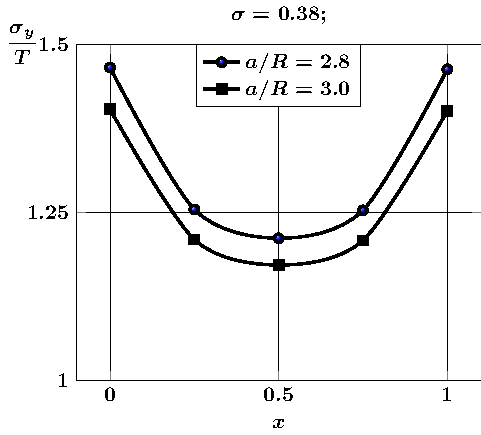
\includegraphics[width=7.6cm]{periodic-spheres-cav27-a-t2-sig_y.pdf}
\caption{Напряжения $\sigma_y/T$ на линии $AB$ в зависимости от расстояния между полостями при двуосном растяжении
\label{f:11:7}}}
\end{figure}

\begin{figure}[h!]
\centering\footnotesize
\parbox[b]{7.5cm}{\centering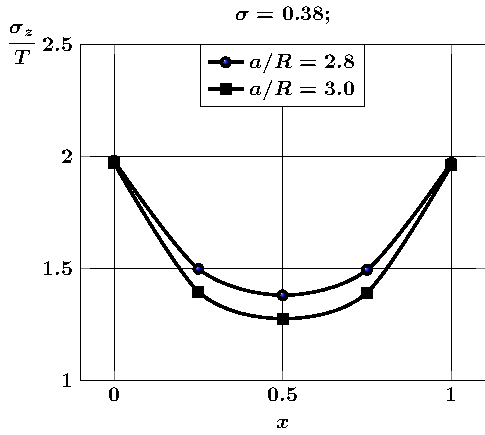
\includegraphics[width=7.6cm]{periodic-spheres-cav27-a-t1-sig_z.pdf}
\caption{Напряжения $\sigma_z/T$ на линии $AB$ в зависимости от расстояния между полостями при одноосном растяжении
\label{f:11:8}}}\hfil\hfil
\parbox[b]{7.5cm}{\centering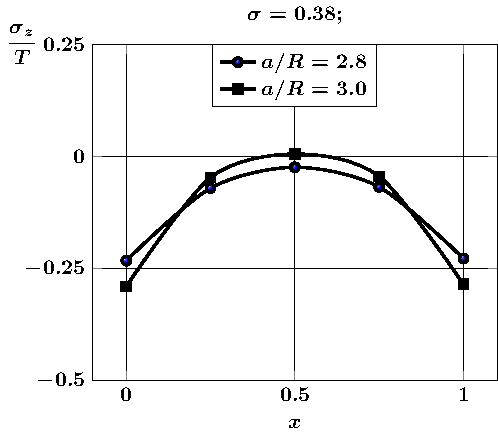
\includegraphics[width=7.8cm]{periodic-spheres-cav27-a-t2-sig_z.pdf}
\caption{Напряжения $\sigma_z/T$ на линии $AB$ в зависимости от расстояния между полостями при двуосном растяжении
\label{f:11:9}}}
\end{figure}

\begin{table}[h!]
\centering
\caption{\centering Сравнение напряжений для разного количества полостей периодической~структуры}
$
\begin{array}{|c|c|c|c|}
\hline
\text{Кол-во полостей} & \sigma_x/T & \sigma_y/T & \sigma_z/T \\
\hline
27 & 0.27904 & 0.10871 & 1.27536 \\
\hline
125 & 0.27934 & 0.11061 & 1.27775 \\
\hline
\end{array}
$
\label{t:11:1}
\end{table}

В табл.~\ref{t:11:1} приведено сравнение нормальных напряжений в средней точке отрезка $AB$ для разного количества (27 и 125) полостей периодической структуры. Из таблицы видно, что увеличение числа полостей практически не меняет значения напряжений.

\begin{figure}[h!]
\centering\footnotesize
\parbox[b]{7.5cm}{\centering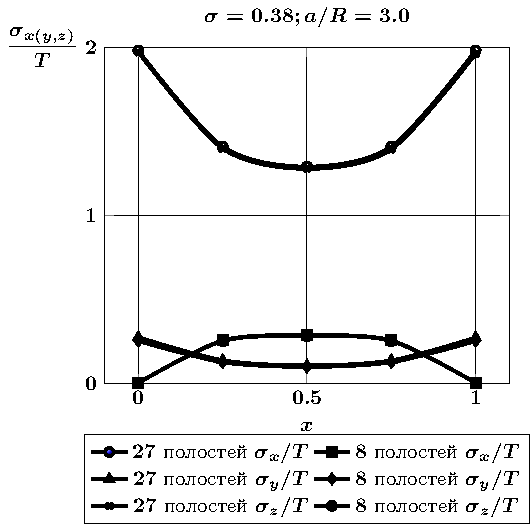
\includegraphics[width=7.8cm]{spheres-cav27-8-a30-t1.pdf}
\caption{Сравнение напряжения на линии $AB$ для периодической и тетрагональной структур при одноосном растяжении
\label{f:11:10}}}\hfil\hfil
\parbox[b]{7.5cm}{\centering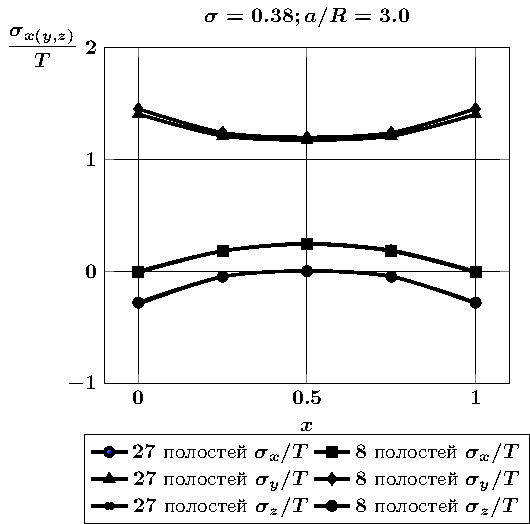
\includegraphics[width=7.8cm]{spheres-cav27-8-a30-t2.pdf}
\caption{Сравнение напряжения на линии $AB$ для периодической и тетрагональной структур при двуосном растяжении
\label{f:11:11}}}
\end{figure}

На рис.~\ref{f:11:10}, \ref{f:11:11} представлено сравнение нормальных напряжений на линии $AB$ для периодической (27 полостей) и тетрагональной (8 полостей) структур при одноосном и двуосном растяжениях упругого пространства. Графики показывают, что все рассмотренные пары напряжений практически не отличаются друг от друга.

\section[Упругое пространство с периодической системой сферических включений]{Упругое пространство с периодической системой сферических включений\sectionmark{Упругое пространство с периодической системой сферических включений}}\sectionmark{Упругое пространство с периодической системой сферических включений}

Рассмотрим упругое пространство $\Omega$ и бесконечную систему сферических включений $\{\omega_{\alpha\beta\gamma}\}_{\alpha,\beta,\gamma=-\infty}^\infty$, центры которых расположены в узлах $\{O_{\alpha\beta\gamma}\}_{\alpha,\beta,\gamma=-\infty}^\infty$ кубической периодической решетки со стороной $a$. Декартовыми координатами узлов решетки будут упорядоченные наборы чисел $\{(\alpha a,\beta a,\gamma a);\,\alpha,\beta,\gamma\in\mathbb{Z}\}$. Радиусы полостей обозначим через $R$. Выполним линейное упорядочение узлов таким же образом, как в предыдущем параграфе.\sloppy

В новой нумерации точка $O_{\alpha,\beta,\gamma}$ обозначается через $O_j$ (см.~рис.~\ref{f:11:1}). С каждой точкой $O_j$ свяжем локальные декартовую $(x_j,y_j,z_j)$ и сонаправленную с ней сферическую системы координат $(r_j,\theta_j,\varphi_j)$. Считается, что декартовые системы координат с началами в точках $O_j$ сонаправлены.

Будем рассматривать задачу упругого деформирования пространства со сферическими включениями под действием нагрузки, приложенной на бесконечности (одноосное, двуосное или всестороннее растяжения упругого пространства).

Соотношения между координатами можно описать формулами~\eqref{eq:11:1}, \eqref{eq:11:2}.

Предполагается, что упругие постоянные включений равны $(\sigma_j,G_j)$. Упругие постоянные матрицы будем считать равными $(\sigma,G)$.

Граничные условия в рассматриваемой задаче представляют собой условия сопряжения полей перемещений и напряжений на поверхностях $\Gamma_j$. Для того, чтобы их записать, представим вектор перемещений в упругом пространстве в виде

\begin{equation}
{\bf{U}} = \left\{ {\begin{array}{*{20}{l}}
{{\bf{\tilde U}}_j^ - ,\quad \left( {x,y,z} \right) \in \omega_j,}\\
{{{{\bf{\tilde U}}}^ + } + {{\bf{U}}_0},\quad \left( {x,y,z} \right) \in\Omega\backslash {\bigcup\limits_j\omega_j},}
\end{array}} \right.
\label{eq:11:23}
\end{equation}

\noindent где $\omega_j = \left\{ {\left( {{r_j},{\theta _j},{\varphi _j}} \right):\, {r_j} < {R_j}} \right\}$. Тогда условия сопряжения принимают следующий вид:

\begin{equation}
\left( {{{{\bf{\tilde U}}}^ + } + {{\bf{U}}_0}} \right){|_{{\Gamma _j}}} = {\bf{\tilde U}}_j^ - {|_{{\Gamma _j}}};
\label{eq:11:24}
\end{equation}

\begin{equation}
\left( {{\bf{F\tilde U^+}} + {\bf{F}}{{\bf{U}}_0}} \right){|_{{\Gamma _j}}} = {\bf{F}}{{\bf{\tilde U^-}}_j}{|_{{\Gamma _j}}},\qquad {\kern 1pt} j = 1,{\mkern 1mu} {\kern 1pt} 2,\dots.
\label{eq:11:25}
\end{equation}

\noindent Условия на бесконечности задаются формулами~\eqref{eq:11:1a}~--- \eqref{eq:11:3a}.

Решение задачи будем искать в виде

\begin{equation}
{\bf{\tilde U^+}} = \sum\limits_{j = 1}^\infty {\sum\limits_{s = 1}^3 {\sum\limits_{n = 0}^\infty  {\sum\limits_{m=-n}^{n} {a_{s,n,m}^{(j)}} } } } {\bf{\tilde U}}_{s,n,m}^{ + (4)}\left( {{r_j},{\theta _j},{\varphi _j}} \right),
\label{eq:11:26}
\end{equation}

\begin{equation}
\mathbf{\tilde U}_j^- = {\sum\limits_{s = 1}^3 {\sum\limits_{n = 0}^\infty  {\sum\limits_{m=-n}^{n} {b_{s,n,m}^{(j)}} } } } {\bf{\tilde U}}_{s,n,m}^{ - (4)}\left( {{r_j},{\theta _j},{\varphi _j}} \right),
\label{eq:11:27}
\end{equation}

\noindent где $G$, $\sigma$~--- модуль сдвига и коэффициент Пуассона упругого пространства; $a_{s,n,m}^{(j)}$, $b_{s,n,m}^{(j)}$~--- неизвестные коэффициенты; перемещения $\mathbf{\tilde U}_{s,n,m}^{\pm(4)}$ приведены в формулах~\eqref{eq:1:89b}~--- \eqref{eq:1:99b}.

Для представления вектора перемещений $\mathbf{\tilde U}^+$ в системах координат с началами $O_j$ можем использовать формулу~\eqref{eq:11:10}.

В силу периодичности задачи вклад каждого слагаемого в формулах~\eqref{eq:11:26}, \eqref{eq:11:27} будет одинаковым, поэтому можно считать, что $a_{s,n,m}^{(j)}=\\=a_{s,n,m}$, $b_{s,n,m}^{(j)}=b_{s,n,m}$.

После удовлетворения условиям~\eqref{eq:11:24}, \eqref{eq:11:25} получаем бесконечную систему линейных алгебраических уравнений относительно неизвестных $a_{s,n,m}$, $b_{s,n,m}$:

\begin{multline}
\sum\limits_{s=1}^3 a_{s,n,m}\tilde E_{s,n,m}^{+(k)}(\sigma)+\tilde E_{s,n,m}^{-(k)}(\sigma)\sum\limits_{t=1}^3\sum\limits_{k=0}^\infty\sum\limits_{l=-k}^k a_{t,k,l}\sum\limits_{\alpha\neq j}\tilde T_{t,k,l,\alpha}^{s,n,m,j}= \\
=-E_{n,m}^{(k)}+\sum\limits_{s=1}^3 b_{s,n,m}\tilde E_{s,n,m}^{-(k)}(\sigma_j);
\label{eq:11:28}
\end{multline}

\begin{multline}
\sum\limits_{s=1}^3 a_{s,n,m}\tilde F_{s,n,m}^{+(k)}(\sigma)+\tilde F_{s,n,m}^{-(k)}(\sigma)\sum\limits_{t=1}^3\sum\limits_{k=0}^\infty\sum\limits_{l=-k}^k a_{t,k,l}\sum\limits_{\alpha\neq j}\tilde T_{t,k,l,\alpha}^{s,n,m,j}= \\
=F_{n,m}^{(k)}+\frac{G_j}{G}\sum\limits_{s=1}^3 b_{s,n,m}\tilde F_{s,n,m}^{-(k)}(\sigma_j);
\label{eq:11:29}
\end{multline}
$$
n,m \in\mathbb{Z} :\quad n \ge 0,\quad |m| \le n,\quad k =  - 1,{\mkern 1mu} {\kern 1pt} 0,{\mkern 1mu} {\kern 1pt} 1,
$$
где $\tilde E_{s,n,m}^{\pm(k)}$~--- компоненты вектора перемещений на поверхности $r_j=R$; $\tilde F_{s,n,m}^{\pm(k)}$~--- компоненты вектора напряжений на поверхности $r_j=R$, отвечающего вектору перемещения $\tilde U_{s,n,m}^{\pm(4)}$:

$$
\mathbf{\tilde U}_{s,n,m}^{\pm(4)}=\tilde E_{s,n,m}^{\pm(-1)}S_n^{m-1}\mathbf{e}_{-1}+\tilde E_{s,n,m}^{\pm(1)}S_n^{m+1}\mathbf{e}_1+\tilde E_{s,n,m}^{\pm(0)}S_n^m\mathbf{e}_0;
$$

$$
\mathbf{F\tilde U}_{s,n,m}^{\pm(4)}=\tilde F_{s,n,m}^{\pm(-1)}S_n^{m-1}\mathbf{e}_{-1}+\tilde F_{s,n,m}^{\pm(1)}S_n^{m+1}\mathbf{e}_1+\tilde F_{s,n,m}^{\pm(0)}S_n^m\mathbf{e}_0;
$$

\begin{equation*}
E_{n,m}^{(k)} =\frac{TR}{2G}\delta_{n1}\delta_{m0}\bigg[-\frac{2\sigma}{1+\sigma}\delta_{k,-1}+\frac{\sigma}{1+\sigma}\delta_{k1}+\frac{1}{1+\sigma}\delta_{k0}\bigg],
\label{eq:11:19a}
\end{equation*}

\begin{equation*}
F_{n,m}^{(k)} =  -\frac{T}{2G}{\delta _{n1}}{\delta _{m0}}{\delta _{k0}}\quad\text{(одноосное растяжение)};
\label{eq:11:19}
\end{equation*}

\begin{equation*}
E_{n,m}^{(k)} =\frac{TR}{2G}\delta_{n1}\delta_{m0}\bigg[\frac{2-2\sigma}{1+\sigma}\delta_{k,-1}-\frac{1-\sigma}{1+\sigma}\delta_{k1}-\frac{2\sigma}{1+\sigma}\delta_{k0}\bigg],
\label{eq:11:20a}
\end{equation*}

\begin{equation*}
F_{n,m}^{(k)} =  -\frac{T}{2G}{\delta _{n1}}{\delta _{m0\,}}(2{\delta _{k, - 1}} - {\delta _{k1}})\quad\text{(двуосное растяжение)};
\label{eq:11:20}
\end{equation*}

\begin{equation*}
E_{n,m}^{(k)} =\frac{TR}{2G}\delta_{n1}\delta_{m0}\frac{1-2\sigma}{1+\sigma}\bigg[2\delta_{k,-1}-\delta_{k1}+\delta_{k0}\bigg],
\label{eq:11:21a}
\end{equation*}

\begin{equation*}
F_{n,m}^{(k)} =  -\frac{T}{2G}{\delta _{n1}}{\delta _{m0\,}}(\delta_{k0}+2{\delta _{k, - 1}} - {\delta _{k1}})\quad\text{(всестороннее растяжение)}.
\label{eq:11:21}
\end{equation*}

Явный вид компонент $\tilde E_{s,n,m}^{\pm(k)}$ и $\tilde F_{s,n,m}^{\pm(k)}$ не приводится ввиду их громоздкости. Они получаются из формул~\eqref{eq:1:91}~--- \eqref{eq:1:94}, \eqref{eq:1:89b}~--- \eqref{eq:1:99b}, \eqref{eq:8:f1}~--- \eqref{eq:8:f6}.

\begin{figure}[h!]
\centering\footnotesize
\parbox[b]{7.5cm}{\centering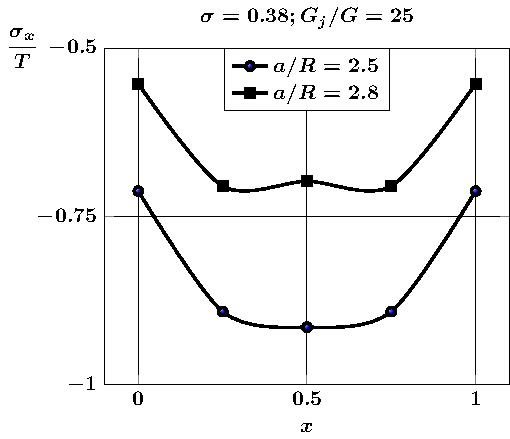
\includegraphics[width=8cm]{periodic-spheres-inc27-a-g25-t1-sig_x.pdf}
\caption{Напряжения $\sigma_x/T$ на линии $AB$ в зависимости от расстояния между включениями при одноосном растяжении
\label{f:11:12}}}\hfil\hfil
\parbox[b]{7.5cm}{\centering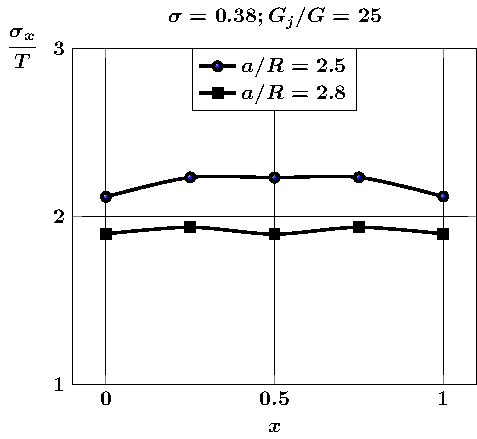
\includegraphics[width=7.6cm]{periodic-spheres-inc27-a-g25-t2-sig_x.pdf}
\caption{Напряжения $\sigma_x/T$ на линии $AB$ в зависимости от расстояния между включениями при двуосном растяжении
\label{f:11:13}}}
\end{figure}

\begin{figure}[h!]
\centering\footnotesize
\parbox[b]{7.5cm}{\centering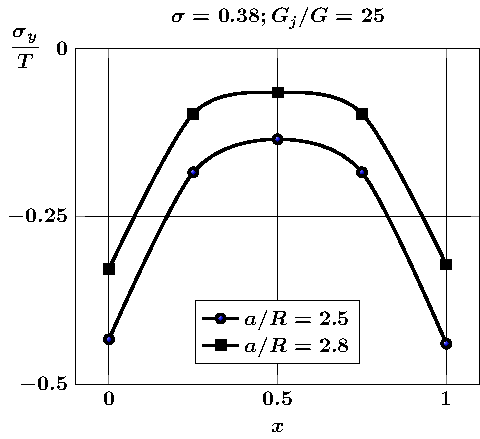
\includegraphics[width=7.6cm]{periodic-spheres-inc27-a-g25-t1-sig_y.pdf}
\caption{Напряжения $\sigma_y/T$ на линии $AB$ в зависимости от расстояния между включениями при одноосном растяжении
\label{f:11:14}}}\hfil\hfil
\parbox[b]{7.5cm}{\centering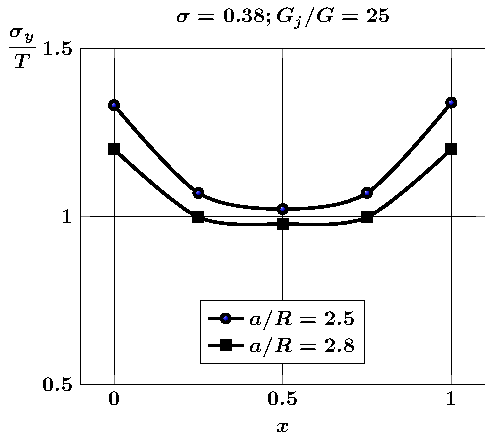
\includegraphics[width=7.6cm]{periodic-spheres-inc27-a-g25-t2-sig_y.pdf}
\caption{Напряжения $\sigma_y/T$ на линии $AB$ в зависимости от расстояния между включениями при двуосном растяжении
\label{f:11:15}}}
\end{figure}

\begin{figure}[h!]
\centering\footnotesize
\parbox[b]{7.5cm}{\centering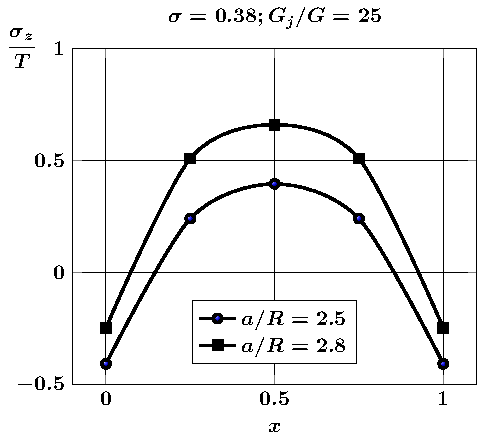
\includegraphics[width=7.5cm]{periodic-spheres-inc27-a-g25-t1-sig_z.pdf}
\caption{Напряжения $\sigma_z/T$ на линии $AB$ в зависимости от расстояния между включениями при одноосном растяжении
\label{f:11:16}}}\hfil\hfil
\parbox[b]{7.5cm}{\centering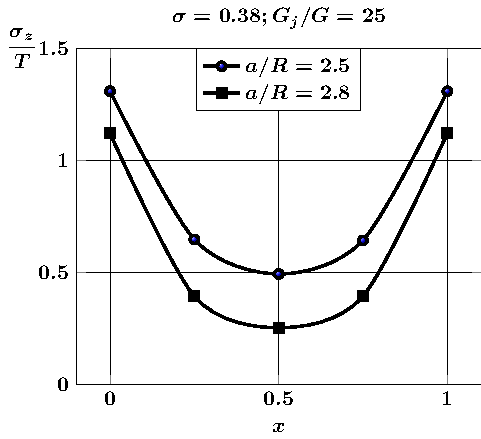
\includegraphics[width=7.5cm]{periodic-spheres-inc27-a-g25-t2-sig_z.pdf}
\caption{Напряжения $\sigma_z/T$ на линии $AB$ в зависимости от расстояния между включениями при двуосном растяжении
\label{f:11:17}}}
\end{figure}

На рис.~\ref{f:11:12}~--- \ref{f:11:17} представлены нормальные напряжения на линии $AB$ в зависимости от расстояния между включениями при одноосном и двуосном растяжениях упругого пространства с периодической системой сферических включений.

При одноосном растяжении основной вклад в тензор напряжений вносят напряжения $\sigma_x/T$ и $\sigma_z/T$. Областью их концентрации является середина отрезка $AB$, где напряжения $\sigma_z/T$~--- растягивающие, а $\sigma_x/T$~--- сжимающие. С приближением включений друг к другу напряжения $\sigma_x/T$ и $\sigma_z/T$ убывают.

При двуосном растяжении основной вклад в тензор напряжений вносят напряжения $\sigma_x/T$, при этом напряжения $\sigma_y/T$ и $\sigma_z/T$ тоже значимы. С приближением включений друг к другу все нормальные напряжения возрастают.

\begin{figure}[h!]
\centering\footnotesize
\parbox[b]{7.5cm}{\centering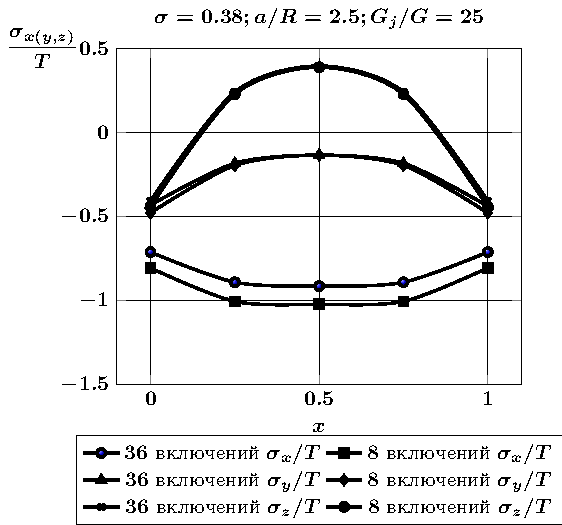
\includegraphics[width=8cm]{spheres-inc27-8-a25-g25-t1.pdf}
\caption{Сравнение напряжений на линии $AB$ для периодической и тетрагональной структур при одноосном растяжении
\label{f:11:18}}}\hfil\hfil
\parbox[b]{7.5cm}{\centering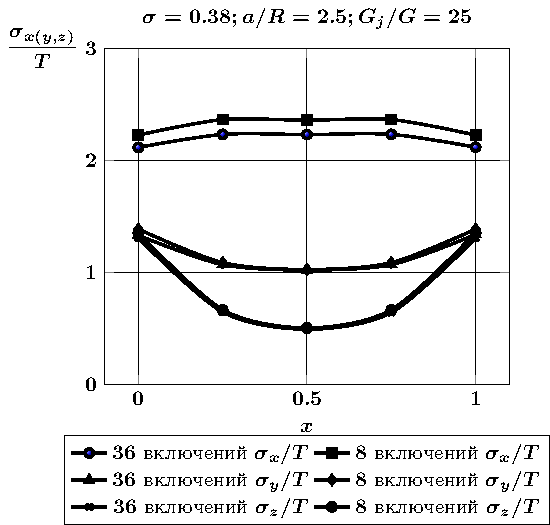
\includegraphics[width=8cm]{spheres-inc27-8-a25-g25-t2.pdf}
\caption{Сравнение напряжений на линии $AB$ для периодической и тетрагональной структур при двуосном растяжении
\label{f:11:19}}}
\end{figure}

На рис.~\ref{f:11:18}, \ref{f:11:19} приведено сравнение нормальных напряжений на линии $AB$ для периодической (36 включений) и тетрагональной (8 включений) структур при одноосном и двуосном растяжении упругого пространства. Графики показывают, что напряжения $\sigma_y/T$ и $\sigma_z/T$ практически совпадают. Небольшое отличие наблюдается в значениях напряжений $\sigma_x/T$ при сохранении общего характера в их распределении.


%***************************************************************************************

\section[Упругое пространство с периодической системой вытянутых сфероидальных полостей]{Упругое пространство с периодической системой вытянутых сфероидальных полостей\sectionmark{Упругое пространство с периодической системой сфероидальных полостей}}\sectionmark{Упругое пространство с периодической системой сфероидальных полостей}

Рассмотрим упругое пространство $\Omega$ и бесконечную систему вытянутых сфероидальных полостей $\{\omega_{\alpha\beta\gamma}\}_{\alpha,\beta,\gamma=-\infty}^\infty$, центры которых расположены в узлах $\{O_{\alpha\beta\gamma}\}_{\alpha,\beta,\gamma=-\infty}^\infty$ кубической периодической решетки со стороной $a$. Декартовыми координатами узлов решетки будут упорядоченные наборы чисел $\{(\alpha a,\beta a,\gamma a);\,\alpha,\beta,\gamma\in\mathbb{Z}\}$. Полуоси полостей обозначим через $d_1$ и $d_2$ ($d_1>d_2$). Выполним линейное упорядочение узлов таким же образом, как в параграфе~6.1.\sloppy

В новой нумерации точка $O_{\alpha,\beta,\gamma}$ обозначается через $O_j$ (рис.~\ref{f:11:1a}).

\begin{figure}[h!]
\centering
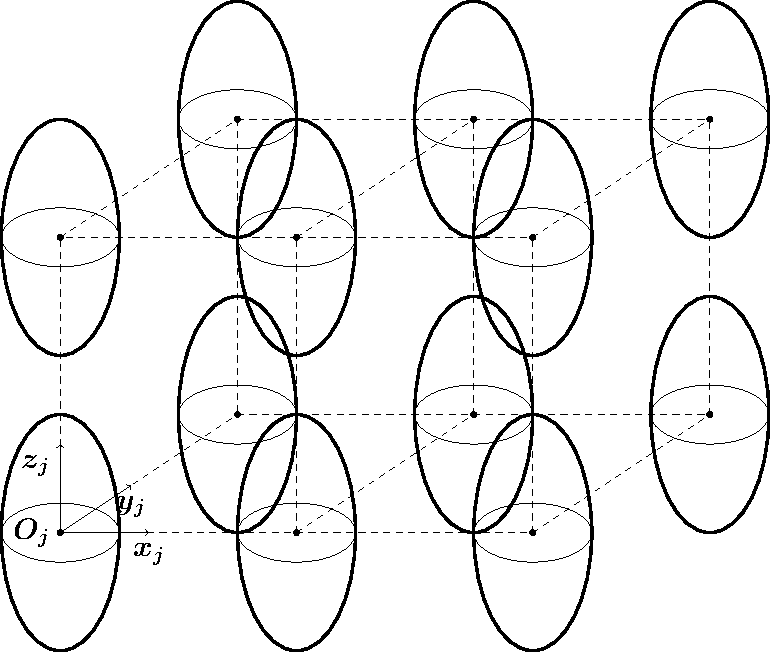
\includegraphics[width=10cm]{cartesian-spheroids-periodic.pdf}
\caption{Периодическая система сфероидальных полостей в упругом пространстве}
\label{f:11:1a}
\end{figure}

С каждой точкой $O_j$ свяжем локальные декартовую $(x_j,y_j,z_j)$ и сонаправленную с ней вытянутую сфероидальную системы координат $(\xi_j,\eta_j,\varphi_j)$. Считается, что декартовые системы координат с началами в точках $O_j$ сонаправлены.

Будем рассматривать задачу упругого деформирования пространства с вытянутыми сфероидальными полостями $\Omega\backslash\bigg\{\bigcup\limits_{\alpha,\beta,\gamma}\omega_{\alpha\beta\gamma}\bigg\}$ под действием нагрузки, приложенной на бесконечности (одноосное, двуосное или всестороннее растяжения упругого пространства). Сфероидальные полости считаются свободными от нагрузки.

Соотношения между координатами можно описать формулами

\begin{equation*}
{x_i} = c\,\mathrm{sh}\xi_j\sin {\eta _i}\cos {\varphi _i},
\end{equation*}

\begin{equation}
{y_i} = c\,\mathrm{sh}\xi_j\sin {\eta _i}\sin {\varphi _i},
\label{eq:11:22}
\end{equation}

\begin{equation*}
{z_i} = c\,\mathrm{ch}\xi_j\cos {\eta _i},
\end{equation*}

\begin{equation}
\left\{ {\begin{array}{*{20}{l}}
{{x_j} = {x_\alpha } + {x_{j\alpha }},}\\
{{y_j} = {y_\alpha } + {y_{j\alpha }},}\\
{{z_j} = {z_\alpha } + {z_{j\alpha }},}
\end{array}} \right.\qquad {\kern 1pt} j \ne \alpha ,\quad j,\alpha  = \overline {1,N},
\label{eq:11:23a}
\end{equation}

\noindent где $\overrightarrow {{O_j}{O_\alpha }}  = \left( {{x_{j\alpha }},{y_{j\alpha }},{z_{j\alpha }}} \right) = \left( {{r_{j\alpha }},{\theta _{j\alpha }},{\varphi _{j\alpha }}} \right)$.

Для определения НДС в рассматриваемом теле необходимо решить краевую задачу для уравнения Ламе относительно неизвестного вектора перемещения   $\mathbf{U}$ с граничными условиями

\begin{equation}
{\bf{FU}}{|_{{\Gamma _j}}} = 0
\end{equation}

\noindent и условиями на бесконечности одного из трех типов

\begin{equation}
{\bf{FU}}{|_{z =  \pm \infty }} =  \pm T{{\bf{e}}_z}\quad\text{(одноосное растяжение)},
\label{eq:11:1a}
\end{equation}

\begin{equation}
{\bf{FU}}{|_{\rho  = \infty }} = T{{\bf{e}}_\rho }\quad\text{(двуосное растяжение)},
\label{eq:11:2a}
\end{equation}

\begin{equation}
{\bf{FU}}{|_{r  = \infty }} = T{{\bf{e}}_r }\quad\text{(всестороннее растяжение)},
\label{eq:11:3a}
\end{equation}

\noindent где $\mathbf{FU}$~--- отвечающий перемещению $\mathbf{U}$ вектор усилий на соответствующей граничной поверхности; ${\Gamma _j} = \left\{ {\left( {{\xi_j},{\eta _j},{\varphi _j}} \right):\,{\xi_j} = {\xi_{0j}}} \right\}$.

Решение задачи будем искать в виде

\begin{equation}
{\bf{U}} = {\bf{\tilde U}} + {{\bf{U}}_0},
\end{equation}

\begin{equation}
{\bf{\tilde U}} = \sum\limits_{j = 1}^\infty {\sum\limits_{s = 1}^3 {\sum\limits_{n = 0}^\infty  {\sum\limits_{m=-n}^{n} {a_{s,n,m}^{(j)}} } } } {\bf{\tilde U}}_{s,n,m}^{ + (5)}\left( {{\xi_j},{\eta _j},{\varphi _j}} \right),
\label{eq:11:24a}
\end{equation}

\begin{equation}
{{\bf{U}}_0} = \frac{T}{{2G}}\left( { - \frac{\sigma }{{1 + \sigma }}{\rho}{{\bf{e}}_{{\rho}}} + \frac{1}{{1 + \sigma }}{z}{{\bf{e}}_z}} \right)\,\text{(одноосное растяжение)},
\label{eq:11:25}
\end{equation}

\begin{equation}
{{\bf{U}}_0} = \frac{T}{{2G}}\left( {\frac{{1 - \sigma }}{{1 + \sigma }}{\rho}{{\bf{e}}_{{\rho}}} - \frac{{2\sigma }}{{1 + \sigma }}{z}{{\bf{e}}_z}} \right)\,\text{(двуосное растяжение)},
\label{eq:11:26}
\end{equation}

\begin{equation}
{{\bf{U}}_0} = \frac{T}{2G}\frac{1-2\sigma}{1+\sigma}\left(\rho\mathbf{e}_\rho+z\mathbf{e}_z\right)\,\text{(всестороннее растяжение)},
\label{eq:11:27}
\end{equation}

\noindent где $G$, $\sigma$~--- модуль сдвига и коэффициент Пуассона упругого пространства; $a_{s,n,m}^{(j)}$~--- неизвестные коэффициенты; перемещения $\mathbf{\tilde U}_{s,n,m}^{+(5)}$ приведены в формулах~\eqref{eq:1:89a}~--- \eqref{eq:1:94a}.

Относительно перемещения $\mathbf{\tilde U}$ граничные условия запишем следующим образом:

\begin{equation}
{\bf{F\tilde U}}{|_{{\Gamma _j}}} =  - {\bf{F}}{{\bf{U}}_0}{|_{{\Gamma _j}}};
\label{eq:11:28a}
\end{equation}

\begin{equation}
{\bf{F\tilde U}}{|_{z =  \pm \infty }} = 0\quad\text{(одноосное растяжение)};
\label{eq:11:29a}
\end{equation}

\begin{equation}
{\bf{F\tilde U}}{|_{\rho  = \infty }} = 0\quad\text{(двуосное растяжение)};
\label{eq:11:30a}
\end{equation}

\begin{equation}
{\bf{F\tilde U}}{|_{r  = \infty }} = 0\quad\text{(всестороннее растяжение)}.
\label{eq:11:30b}
\end{equation}

Вспомогательным перемещениям $\mathbf{U}_0$ отвечают такие напряжения на поверхностях $\Gamma_j$ ($\mathbf{n}_j=\mathbf{e}_{\xi_j}$~--- вектор нормали на поверхности $\Gamma_j$):

\begin{equation}
{\bf{F}}{{\bf{U}}_0} = TH_j\,\mathrm{sh}\xi_j P_1(\cos\eta_j)\mathbf{e}_z\quad\text{(одноосное растяжение)};
\label{eq:11:g1}
\end{equation}

\begin{equation}
{\bf{F}}{{\bf{U}}_0} = -TH_j\,\mathrm{ch}\xi_j P_1^{(1)}(\cos\eta_j)\mathbf{e}_{\rho_j}\quad\text{(двуосное растяжение)};
\label{eq:11:g2}
\end{equation}

\begin{multline}
\mathbf{FU}_0=TH_j\bigg[-\mathrm{ch}\xi_j P_1^{(1)}(\cos\eta_j)\mathbf{e}_{\rho_j}+ \\
+\mathrm{sh}\xi_jP_1(\cos\eta_j)\mathbf{e}_z\bigg]\,\text{(всестороннее растяжение)}.
\label{eq:11:g3}
\end{multline}

Используя теоремы сложения~\eqref{eq:1:100t}, перемещение $\mathbf{\tilde U}$ можно записать полностью в системе координат с началом в точке $O_j$:

\begin{multline}
{\bf{\tilde U}} = \sum\limits_{s = 1}^3 {\sum\limits_{n = 0}^\infty  {\sum\limits_{m =  - n }^{n } {a_{s,n,m}^{(j)}} } } {\bf{\tilde U}}_{s,n,m}^{ +(5)}\left( {{\xi_j},{\eta _j},{\varphi _j}} \right) + \\
+ \sum\limits_{s=1}^3\sum\limits_{n = 0}^\infty\sum\limits_{m =  - n }^{n }{\bf{\tilde U}}_{s,n,m}^{ - (5)}\left( {{\xi_j},{\eta _j},{\varphi _j}} \right)\sum\limits_{\alpha  \ne j}\sum\limits_{t=1}^3\sum\limits_{k = 0}^\infty\mathop \sum \limits_{l =  - k}^{k}\tilde T_{t,k,l,\alpha}^{s,n,m,j}a_{t,k,l}^{(\alpha)}.
\label{eq:11:31}
\end{multline}

В силу периодичности задачи вклад каждого слагаемого в формуле~\eqref{eq:11:24a} будет одинаковым, поэтому можно считать, что $a_{s,n,m}^{(j)}=a_{s,n,m}$.

После перехода в формуле~\eqref{eq:11:31} к напряжениям и удовлетворения граничным условиям относительно неизвестных $a_{s,n,m}$ получаем бесконечную систему линейных алгебраических уравнений:

\begin{equation}
\sum\limits_{s=1}^3 a_{s,n,m}\tilde F_{s,n,m}^{+(k)}+\tilde F_{s,n,m}^{-(k)}\sum\limits_{t=1}^3\sum\limits_{k=0}^\infty\sum\limits_{l=-k}^k a_{t,k,l}\sum\limits_{\alpha\neq j}\tilde T_{t,k,l,\alpha}^{s,n,m,j}=F_{n,m}^{(k)};
\label{eq:11:sys}
\end{equation}
$$
n,m \in\mathbb{Z}:\quad n \ge 0,{\mkern 1mu} \quad {\kern 1pt} |m| \le n,\quad {\mkern 1mu} k =  - 1,{\mkern 1mu} {\kern 1pt} 0,{\mkern 1mu} {\kern 1pt} 1;\;\;\;{\mkern 1mu} {\kern 1pt} j = \overline {1,\infty},
$$

\noindent где $\tilde F_{s,n,m}^{\pm(k)}$~--- компоненты вектора напряжений на поверхности $\xi_j=\xi_{j0}$, отвечающего вектору перемещения $\tilde U_{s,n,m}^{\pm(5)}$:

$$
\mathbf{F\tilde U}_{s,n,m}^{\pm(5)}=\frac{H_j}{c}\bigg(\tilde F_{s,n,m}^{\pm(-1)}S_n^{m-1}\mathbf{e}_{-1}+\tilde F_{s,n,m}^{\pm(1)}S_n^{m+1}\mathbf{e}_1+\tilde F_{s,n,m}^{\pm(0)}S_n^m\mathbf{e}_0\bigg);
$$

\begin{figure}[h!]
\centering\footnotesize
\parbox[b]{7.5cm}{\centering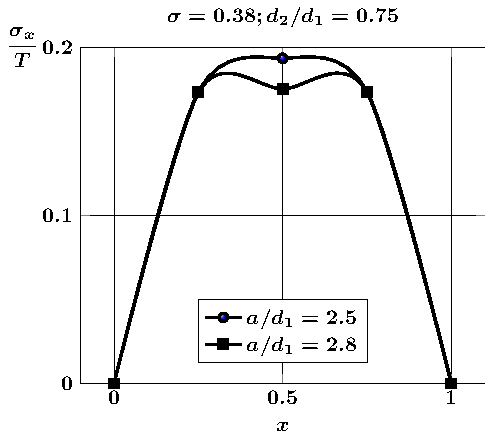
\includegraphics[width=7.6cm]{periodic-cav27-a-d75-t1-sig_x.pdf}
\caption{Напряжения $\sigma_x/T$ на линии $AB$ в зависимости от расстояния между полостями при одноосном растяжении
\label{f:11:20}}}\hfil\hfil
\parbox[b]{7.5cm}{\centering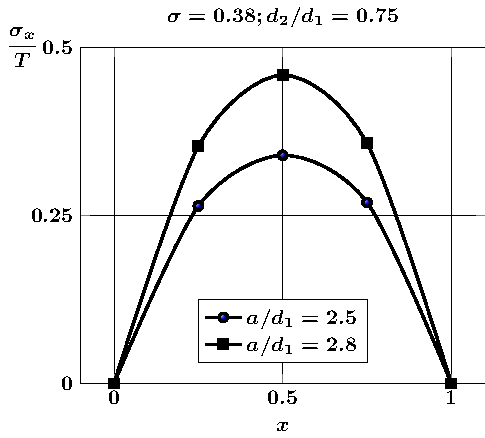
\includegraphics[width=7.6cm]{periodic-cav27-a-d75-t2-sig_x.pdf}
\caption{Напряжения $\sigma_x/T$ на линии $AB$ в зависимости от расстояния между полостями при двуосном растяжении
\label{f:11:21}}}
\end{figure}

\begin{figure}[h!]
\centering\footnotesize
\parbox[b]{7.5cm}{\centering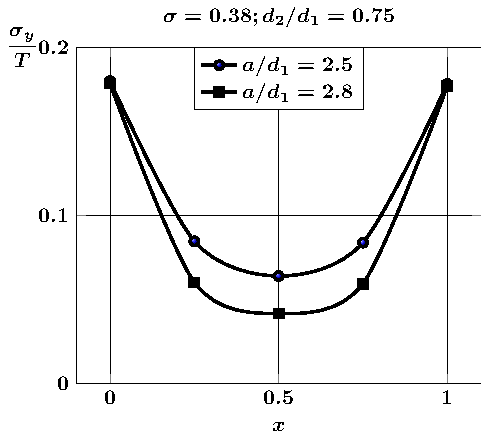
\includegraphics[width=7.6cm]{periodic-cav27-a-d75-t1-sig_y.pdf}
\caption{Напряжения $\sigma_y/T$ на линии $AB$ в зависимости от расстояния между полостями при одноосном растяжении
\label{f:11:22}}}\hfil\hfil
\parbox[b]{7.5cm}{\centering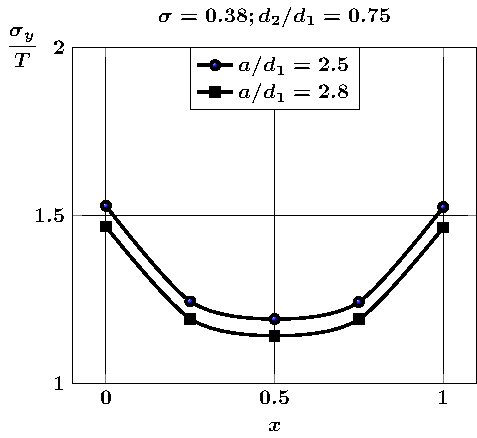
\includegraphics[width=7.6cm]{periodic-cav27-a-d75-t2-sig_y.pdf}
\caption{Напряжения $\sigma_y/T$ на линии $AB$ в зависимости от расстояния между полостями при двуосном растяжении
\label{f:11:23}}}
\end{figure}

\begin{equation*}
F_{n,m}^{(k)} =  -\frac{Td_2}{2G}{\delta _{n1}}{\delta _{m0}}{\delta _{k0}}\quad\text{(одноосное растяжение)},
\label{eq:11:19}
\end{equation*}

\begin{equation*}
F_{n,m}^{(k)} =  -\frac{Td_1}{2G}{\delta _{n1}}{\delta _{m0\,}}(2{\delta _{k, - 1}} - {\delta _{k1}})\quad\text{(двуосное растяжение)},
\label{eq:11:20}
\end{equation*}

\begin{equation*}
F_{n,m}^{(k)} =  -\frac{T}{2G}{\delta _{n1}}{\delta _{m0\,}}(\delta_{k0}d_2+2{\delta _{k, - 1}}d_1 - {\delta _{k1}}d_1)\quad\text{(всестороннее растяжение)}.
\label{eq:11:21}
\end{equation*}

Явный вид компонент $\tilde F_{s,n,m}^{\pm(k)}$ не приводится ввиду их громоздкости. Они получаются из формул~\eqref{eq:1:89a}~--- \eqref{eq:1:99a}, \eqref{eq:9:f1}~--- \eqref{eq:9:f3}.

\begin{figure}[h!]
\centering\footnotesize
\parbox[b]{7.5cm}{\centering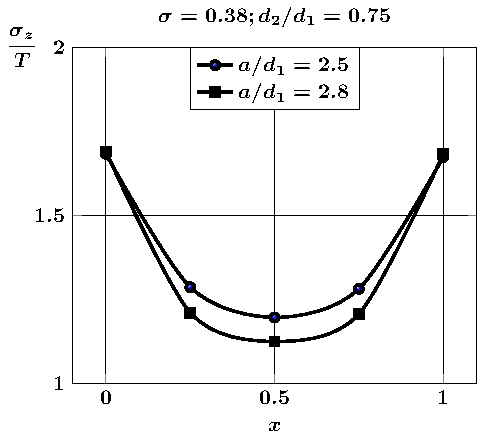
\includegraphics[width=7.6cm]{periodic-cav27-a-d75-t1-sig_z.pdf}
\caption{Напряжения $\sigma_z/T$ на линии $AB$ в зависимости от расстояния между полостями при одноосном растяжении
\label{f:11:24}}}\hfil\hfil
\parbox[b]{7.5cm}{\centering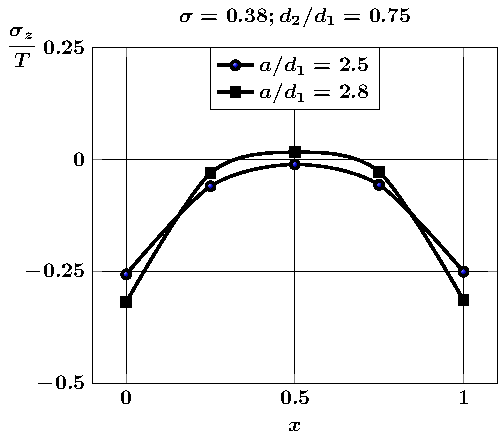
\includegraphics[width=7.8cm]{periodic-cav27-a-d75-t2-sig_z.pdf}
\caption{Напряжения $\sigma_z/T$ на линии $AB$ в зависимости от расстояния между полостями при двуосном растяжении
\label{f:11:25}}}
\end{figure}

\begin{figure}[h!]
\centering\footnotesize
\parbox[b]{7.5cm}{\centering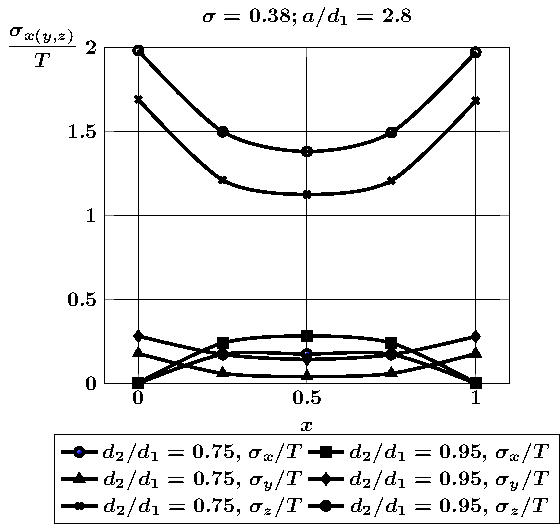
\includegraphics[width=8cm]{periodic-cav27-d-a28-t1.pdf}
\caption{Сравнение напряжений на линии $AB$ в зависимости от формы сфероидальной полости при одноосном растяжении
\label{f:11:31}}}\hfil\hfil
\parbox[b]{7.5cm}{\centering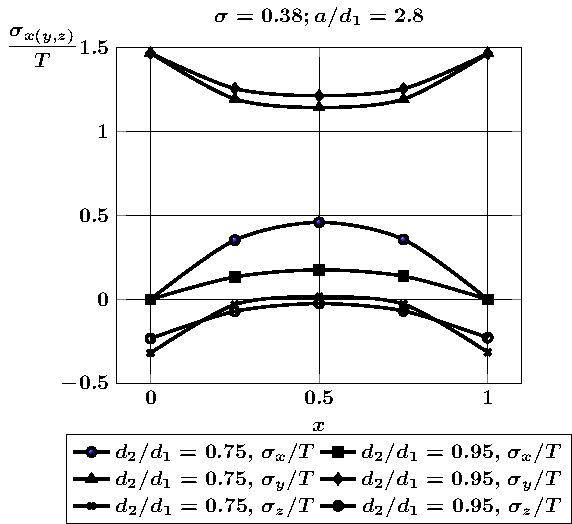
\includegraphics[width=8cm]{periodic-cav27-d-a28-t2.pdf}
\caption{Сравнение напряжений на линии $AB$ в зависимости от формы сфероидальной полости при двуосном растяжении
\label{f:11:32}}}
\end{figure}

На рис.~\ref{f:11:20}~--- \ref{f:11:25} приведены нормальные напряжения на линии $AB$ в зависимости от относительного расстояния $a/d_1$ между полостями при одноосном и двуосном растяжениях упругого пространства при $\sigma=0.38$ и $d_2/d_1=0.75$.

При одноосном растяжении основной вклад в тензор напряжений вносят напряжения $\sigma_z/T$. Областью их концентрации являются границы полостей. С приближением полостей друг к другу эти напряжения возрастают.

При двуосном растяжении подобным поведением характеризуются напряжения $\sigma_y/T$.

На рис.~\ref{f:11:31}, \ref{f:11:32} представлено сравнение нормальных напряжений на линии $AB$ в зависимости от формы сфероидальных полостей при одноосном и двуосном растяжениях упругого пространства.

Заметное отличие наблюдается в значениях напряжений $\sigma_z/T$ при одноосном растяжении и $\sigma_x/T$~--- при двуосном. В случае одноосного растяжения для полости, близкой по форме к сферической, все приведенные напряжения больше, чем для вытянутой сфероидальной полости. В случае двуосного растяжения для напряжения $\sigma_x/T$ наблюдается обратная картина.

\begin{table}[h!]
\centering
\caption{\centering Сравнение напряжений для разного количества полостей~периодической~структуры}
$
\begin{array}{|c|c|c|c|}
\hline
\text{Кол-во полостей} & \sigma_x/T & \sigma_y/T & \sigma_z/T \\
\hline
27 & 0.1751 & 0.04153 & 1.1248 \\
\hline
125 & 0.1752 & 0.04261 & 1.1261 \\
\hline
\end{array}
$
\label{t:11:2}
\end{table}

В табл.~\ref{t:11:2} приведено сравнение нормальных напряжений в средней точке отрезка $AB$ для разного количества (27 и 125) сфероидальных полостей периодической структуры. Из таблицы видно, что увеличение числа полостей практически не меняет значения напряжений.

\section[Упругое пространство с периодической системой вытянутых сфероидальных включений]{Упругое пространство с периодической системой вытянутых сфероидальных включений\sectionmark{Упругое пространство с периодической системой сфероидальных включений}}\sectionmark{Упругое пространство с периодической системой сфероидальных включений}

Рассмотрим упругое пространство $\Omega$ и бесконечную систему вытянутых сфероидальных включений $\{\omega_{\alpha\beta\gamma}\}_{\alpha,\beta,\gamma=-\infty}^\infty$, центры которых расположены в узлах $\{O_{\alpha\beta\gamma}\}_{\alpha,\beta,\gamma=-\infty}^\infty$ кубической периодической решетки со стороной $a$. Декартовыми координатами узлов решетки будут упорядоченные наборы чисел $\{(\alpha a,\beta a,\gamma a);\,\alpha,\beta,\gamma\in\mathbb{Z}\}$. Полуоси включений обозначим через $d_1$ и $d_2$ ($d_1>d_2$). Выполним линейное упорядочение узлов таким же образом, как в параграфе 6.1.\sloppy

В новой нумерации точка $O_{\alpha,\beta,\gamma}$ обозначается через $O_j$ (см.~рис.~\ref{f:11:1a}). С каждой точкой $O_j$ свяжем локальные декартовую $(x_j,y_j,z_j)$ и сонаправленную с ней вытянутую сфероидальную системы координат $(\xi_j,\eta_j,\varphi_j)$. Считается, что декартовые системы координат с началами в точках $O_j$ сонаправлены.

Будем рассматривать задачу упругого деформирования пространства с вытянутыми сфероидальными включениями под действием нагрузки, приложенной на бесконечности (одноосное, двуосное или всестороннее растяжения упругого пространства).

Соотношения между координатами можно описать формулами~\eqref{eq:11:22}, \eqref{eq:11:23a}.

Предполагается, что упругие постоянные включений равны $(\sigma_j,G_j)$. Упругие постоянные матрицы будем считать равными $(\sigma,G)$.

Граничные условия в рассматриваемой задаче представляют собой условия сопряжения полей перемещений и напряжений на поверхностях $\Gamma_j$. Для того, чтобы их записать, представим вектор перемещений в упругом пространстве в виде

\begin{equation}
{\bf{U}} = \left\{ {\begin{array}{*{20}{l}}
{{\bf{\tilde U}}_j^ - ,\quad \left( {x,y,z} \right) \in \omega_j,}\\
{{{{\bf{\tilde U}}}^ + } + {{\bf{U}}_0},\quad \left( {x,y,z} \right) \in\Omega\backslash {\bigcup\limits_j\omega_j},}
\end{array}} \right.
\label{eq:11:23i}
\end{equation}

\noindent где $\omega_j = \left\{ {\left( {{\xi_j},{\eta _j},{\varphi _j}} \right):\, {\xi_j} < {\xi_{0j}}} \right\}$. Тогда условия сопряжения принимают следующий вид:

\begin{equation}
\left( {{{{\bf{\tilde U}}}^ + } + {{\bf{U}}_0}} \right){|_{{\Gamma _j}}} = {\bf{\tilde U}}_j^ - {|_{{\Gamma _j}}},
\label{eq:11:24i}
\end{equation}

\begin{equation}
\left( {{\bf{F\tilde U^+}} + {\bf{F}}{{\bf{U}}_0}} \right){|_{{\Gamma _j}}} = {\bf{F}}{{\bf{\tilde U^-}}_j}{|_{{\Gamma _j}}},\qquad {\kern 1pt} j = 1,{\mkern 1mu} {\kern 1pt} 2,\dots.
\label{eq:11:25i}
\end{equation}

\noindent Условия на бесконечности задаются формулами~\eqref{eq:11:g1}~--- \eqref{eq:11:g3}.

Решение задачи будем искать в виде

\begin{equation}
{\bf{\tilde U^+}} = \sum\limits_{j = 1}^\infty {\sum\limits_{s = 1}^3 {\sum\limits_{n = 0}^\infty  {\sum\limits_{m=-n}^{n} {a_{s,n,m}^{(j)}} } } } {\bf{\tilde U}}_{s,n,m}^{ + (5)}\left( {{\xi_j},{\eta _j},{\varphi _j}} \right),
\label{eq:11:26i}
\end{equation}

\begin{equation}
\mathbf{\tilde U}_j^- = {\sum\limits_{s = 1}^3 {\sum\limits_{n = 0}^\infty  {\sum\limits_{m=-n}^{n} {b_{s,n,m}^{(j)}} } } } {\bf{\tilde U}}_{s,n,m}^{ - (5)}\left( {{\xi_j},{\eta _j},{\varphi _j}} \right),
\label{eq:11:27i}
\end{equation}

\noindent где $G$, $\sigma$~--- модуль сдвига и коэффициент Пуассона упругого пространства; $a_{s,n,m}^{(j)}$, $b_{s,n,m}^{(j)}$~--- неизвестные коэффициенты; перемещения $\mathbf{\tilde U}_{s,n,m}^{\pm(5)}$ приведены в формулах~\eqref{eq:1:89a}~--- \eqref{eq:1:99a}.

Для представления вектора перемещений $\mathbf{\tilde U}^+$ в системах координат с началами $O_j$ можем использовать формулу~\eqref{eq:11:31}.

В силу периодичности задачи вклад каждого слагаемого в формулах~\eqref{eq:11:26i}, \eqref{eq:11:27i} будет одинаковым, поэтому можно считать, что $a_{s,n,m}^{(j)}=\\=a_{s,n,m}$, $b_{s,n,m}^{(j)}=b_{s,n,m}$.

После перехода к напряжениям в формуле~\eqref{eq:11:31} и удовлетворения условиям~\eqref{eq:11:24i}, \eqref{eq:11:25i} получаем бесконечную систему линейных алгебраических уравнений относительно неизвестных $a_{s,n,m}$, $b_{s,n,m}$:

\begin{multline}
\sum\limits_{s=1}^3 a_{s,n,m}\tilde E_{s,n,m}^{+(k)}(\sigma)+\tilde E_{s,n,m}^{-(k)}(\sigma)\sum\limits_{t=1}^3\sum\limits_{k=0}^\infty\sum\limits_{l=-k}^k a_{t,k,l}\sum\limits_{\alpha\neq j}\tilde T_{t,k,l,\alpha}^{s,n,m,j}= \\
=-E_{n,m}^{(k)}+\sum\limits_{s=1}^3 b_{s,n,m}\tilde E_{s,n,m}^{-(k)}(\sigma_j);
\label{eq:11:28i}
\end{multline}

\begin{multline}
\sum\limits_{s=1}^3 a_{s,n,m}\tilde F_{s,n,m}^{+(k)}(\sigma)+\tilde F_{s,n,m}^{-(k)}(\sigma)\sum\limits_{t=1}^3\sum\limits_{k=0}^\infty\sum\limits_{l=-k}^k a_{t,k,l}\sum\limits_{\alpha\neq j}\tilde T_{t,k,l,\alpha}^{s,n,m,j}= \\
=F_{n,m}^{(k)}+\frac{G_j}{G}\sum\limits_{s=1}^3 b_{s,n,m}\tilde F_{s,n,m}^{-(k)}(\sigma_j);
\label{eq:11:29i}
\end{multline}

\begin{equation}
n,m \in\mathbb{Z} :\quad n \ge 0,\quad |m| \le n,\quad k =  - 1,{\mkern 1mu} {\kern 1pt} 0,{\mkern 1mu} {\kern 1pt} 1,
\end{equation}

\noindent где $\tilde E_{s,n,m}^{\pm(k)}$~--- компоненты вектора перемещений на поверхности $\xi_j=\xi_{0j}$; $\tilde F_{s,n,m}^{\pm(k)}$~--- компоненты вектора напряжений на поверхности $\xi_j=\xi_{0j}$, отвечающего вектору перемещения $\tilde U_{s,n,m}^{\pm(5)}$:

$$
\mathbf{\tilde U}_{s,n,m}^{\pm(5)}=\tilde E_{s,n,m}^{\pm(-1)}S_n^{m-1}\mathbf{e}_{-1}+\tilde E_{s,n,m}^{\pm(1)}S_n^{m+1}\mathbf{e}_1+\tilde E_{s,n,m}^{\pm(0)}S_n^m\mathbf{e}_0;
$$

$$
\mathbf{F\tilde U}_{s,n,m}^{\pm(5)}=\frac{H_j}{c}\bigg(\tilde F_{s,n,m}^{\pm(-1)}S_n^{m-1}\mathbf{e}_{-1}+\tilde F_{s,n,m}^{\pm(1)}S_n^{m+1}\mathbf{e}_1+\tilde F_{s,n,m}^{\pm(0)}S_n^m\mathbf{e}_0\bigg);
$$

\begin{equation*}
E_{n,m}^{(k)} =\frac{Tc}{2G}\delta_{n1}\delta_{m0}\bigg[-\frac{2\sigma}{1+\sigma}\,\mathrm{sh}\xi_{0j}\delta_{k,-1}+\frac{\sigma}{1+\sigma}\,\mathrm{sh}\xi_{0j}\delta_{k1}+\frac{1}{1+\sigma}\,\mathrm{ch}\xi_{0j}\delta_{k0}\bigg],
\end{equation*}

\begin{equation*}
F_{n,m}^{(k)} =  -\frac{Td_2}{2G}{\delta _{n1}}{\delta _{m0}}{\delta _{k0}}\quad\text{(одноосное растяжение)};
\end{equation*}

\begin{equation*}
E_{n,m}^{(k)} =\frac{Tc}{2G}\delta_{n1}\delta_{m0}\bigg[\frac{2-2\sigma}{1+\sigma}\,\mathrm{sh}\xi_{0j}\delta_{k,-1}-\frac{1-\sigma}{1+\sigma}\,\mathrm{sh}\xi_{0j}\delta_{k1}-\frac{2\sigma}{1+\sigma}\,\mathrm{ch}\xi_{0j}\delta_{k0}\bigg],
\end{equation*}

\begin{figure}[h!]
\centering\footnotesize
\parbox[b]{7.5cm}{\centering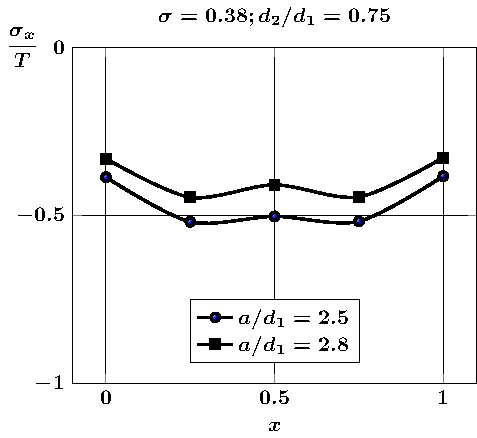
\includegraphics[width=7.6cm]{periodic-inc27-a-d75-g25-t1-sig_x.pdf}
\caption{Напряжения $\sigma_x/T$ на линии $AB$ в зависимости от расстояния между включениями при одноосном растяжении
\label{f:11:25}}}\hfil\hfil
\parbox[b]{7.5cm}{\centering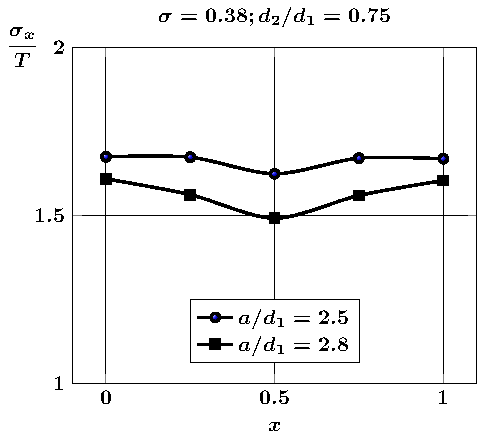
\includegraphics[width=7.6cm]{periodic-inc27-a-d75-g25-t2-sig_x.pdf}
\caption{Напряжения $\sigma_x/T$ на линии $AB$ в зависимости от расстояния между включениями при двуосном растяжении
\label{f:11:26}}}
\end{figure}

\begin{figure}[h!]
\centering\footnotesize
\parbox[b]{7.5cm}{\centering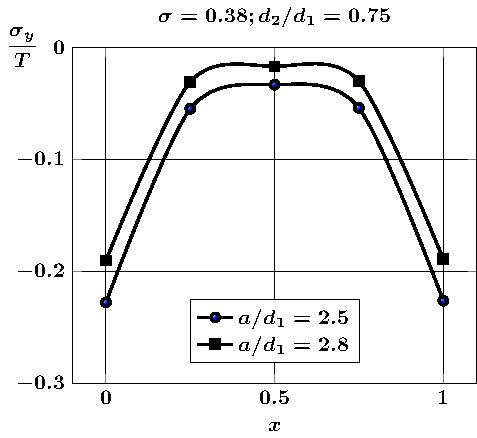
\includegraphics[width=7.6cm]{periodic-inc27-a-d75-g25-t1-sig_y.pdf}
\caption{Напряжения $\sigma_y/T$ на линии $AB$ в зависимости от расстояния между включениями при одноосном растяжении
\label{f:11:27}}}\hfil\hfil
\parbox[b]{7.5cm}{\centering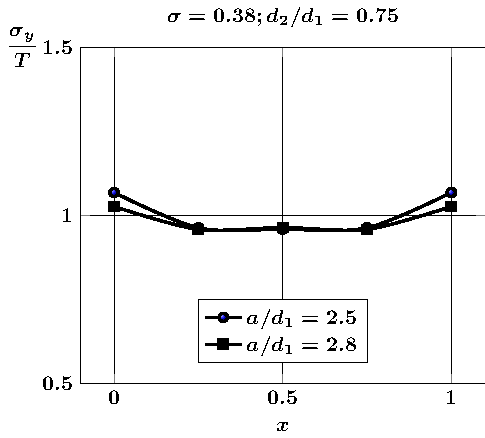
\includegraphics[width=7.6cm]{periodic-inc27-a-d75-g25-t2-sig_y.pdf}
\caption{Напряжения $\sigma_y/T$ на линии $AB$ в зависимости от расстояния между включениями при двуосном растяжении
\label{f:11:28}}}
\end{figure}

\begin{equation*}
F_{n,m}^{(k)} =  -\frac{Td_1}{2G}{\delta _{n1}}{\delta _{m0\,}}(2{\delta _{k, - 1}} - {\delta _{k1}})\quad\text{(двуосное растяжение)};
\end{equation*}

\begin{equation*}
E_{n,m}^{(k)} =\frac{Tc}{2G}\delta_{n1}\delta_{m0}\frac{1-2\sigma}{1+\sigma}\bigg[2\,\mathrm{sh}\xi_{0j}\delta_{k,-1}-\mathrm{sh}\xi_{0j}\delta_{k1}+\mathrm{ch}\xi_{0j}\delta_{k0}\bigg],
\end{equation*}

\begin{equation*}
F_{n,m}^{(k)} =  -\frac{T}{2G}{\delta _{n1}}{\delta _{m0\,}}(d_2\delta_{k0}+2d_1{\delta _{k, - 1}} - d_1{\delta _{k1}})\quad\text{(всестороннее растяжение)}.
\end{equation*}

Явный вид компонент $\tilde E_{s,n,m}^{\pm(k)}$ и $\tilde F_{s,n,m}^{\pm(k)}$ не приводится ввиду их громоздкости. Они получаются из формул~\eqref{eq:1:42}~--- \eqref{eq:1:44}, \eqref{eq:1:89a}~--- \eqref{eq:1:99a}, \eqref{eq:9:f1}~--- \eqref{eq:9:f3}.

На рис.~\ref{f:11:25}~--- \ref{f:11:30} приведены нормальные напряжения на линии $AB$ в зависимости от относительного расстояния между включениями при одноосном и двуосном растяжениях упругого пространства при $\sigma=0.38$, $\sigma_j=0.21$, $G_j/G=25$, $d_2/d_1=0.75$.

\begin{figure}[h!]
\centering\footnotesize
\parbox[b]{7.5cm}{\centering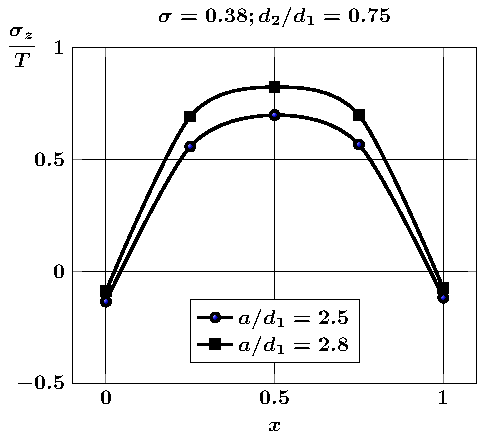
\includegraphics[width=7.6cm]{periodic-inc27-a-d75-g25-t1-sig_z.pdf}
\caption{Напряжения $\sigma_z/T$ на линии $AB$ в зависимости от расстояния между включениями при одноосном растяжении
\label{f:11:29}}}\hfil\hfil
\parbox[b]{7.5cm}{\centering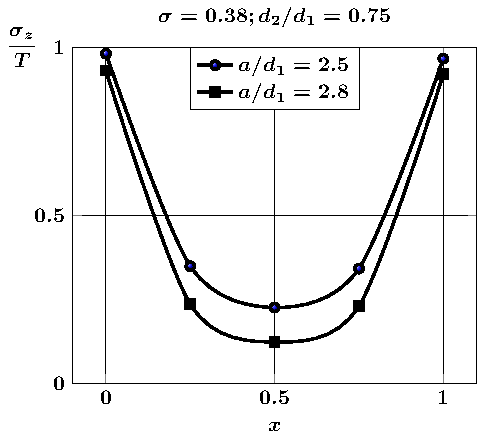
\includegraphics[width=7.6cm]{periodic-inc27-a-d75-g25-t2-sig_z.pdf}
\caption{Напряжения $\sigma_z/T$ на линии $AB$ в зависимости от расстояния между включениями при двуосном растяжении
\label{f:11:30}}}
\end{figure}

\begin{figure}[h!]
\centering\footnotesize
\parbox[b]{7.5cm}{\centering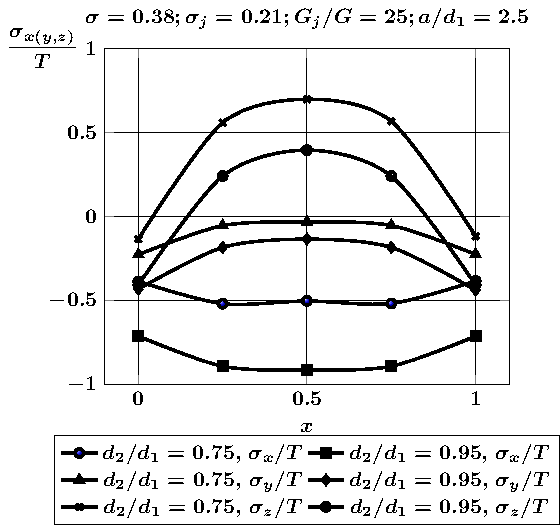
\includegraphics[width=7.8cm]{periodic-inc27-d-a25-g25-t1.pdf}
\caption{Сравнение напряжений на линии $AB$ в зависимости от формы сфероидального включения при одноосном растяжении
\label{f:11:33}}}\hfil\hfil
\parbox[b]{7.5cm}{\centering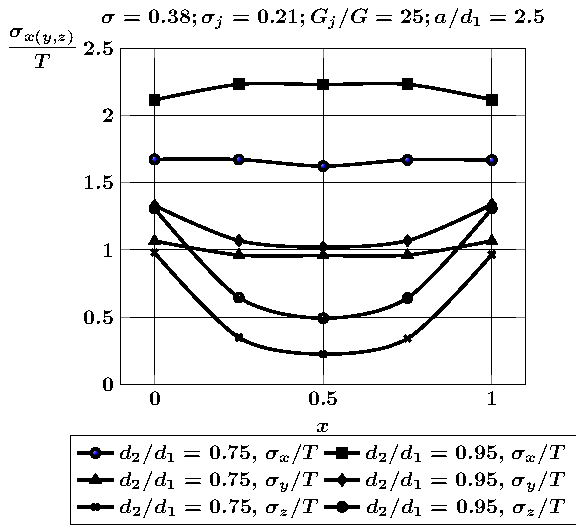
\includegraphics[width=8cm]{periodic-inc27-d-a25-g25-t2.pdf}
\caption{Сравнение напряжений на линии $AB$ в зависимости от формы сфероидального включения при двуосном растяжении
\label{f:11:34}}}
\end{figure}

При одноосном растяжении основной вклад в тензор напряжений вносят напряжения $\sigma_z/T$. Напряжения $\sigma_x/T$ тоже значимы. Характерно, что они являются сжимающими. Область концентрации напряжений $\sigma_z/T$ совпадает с серединой отрезка $AB$. С приближением включений друг к другу эти напряжения убывают.

При двуосном растяжении основной вклад в тензор напряжений вносят напряжения $\sigma_x/T$, однако напряжения $\sigma_y/T$ и $\sigma_z/T$ тоже значимы. Напряжения $\sigma_x/T$ и $\sigma_y/T$ незначительно меняются в пределах отрезка $AB$ и возрастают с приближением полостей друг к другу. Наблюдается сильная концентрация напряжений $\sigma_z/T$ на границе включений.

На рис.~\ref{f:11:33}, \ref{f:11:34} представлено сравнение нормальных напряжений на линии $AB$ в зависимости от формы сфероидальных включений при одноосном и двуосном растяжениях упругого пространства.

Графики показывают, что в случае и одноосного и двуосного растяжений упругого пространства при изменении формы сфероидального включения сохраняется общий характер в распределении напряжений, однако численные значения напряжений существенно отличаются.

%*************************************************************************************

\section[Упругое пространство с периодической системой сжатых сфероидальных полостей]{Упругое пространство с периодической системой сжатых сфероидальных полостей\sectionmark{Упругое пространство с периодической системой сфероидальных полостей}}\sectionmark{Упругое пространство с периодической системой сфероидальных полостей}

Рассмотрим упругое пространство $\Omega$ и бесконечную систему сжатых сфероидальных полостей $\{\omega_{\alpha\beta\gamma}\}_{\alpha,\beta,\gamma=-\infty}^\infty$, центры которых расположены в узлах $\{O_{\alpha\beta\gamma}\}_{\alpha,\beta,\gamma=-\infty}^\infty$ кубической периодической решетки со стороной $a$. Декартовыми координатами узлов решетки будут упорядоченные наборы чисел $\{(\alpha a,\beta a,\gamma a);\,\alpha,\beta,\gamma\in\mathbb{Z}\}$. Полуоси полостей обозначим через $d_1$ и $d_2$ ($d_2>d_1$). Выполним линейное упорядочение узлов таким же образом, как в параграфе~6.1.\sloppy

В новой нумерации точка $O_{\alpha,\beta,\gamma}$ обозначается через $O_j$ (рис.~\ref{f:11:1b}).

\begin{figure}[h!]
\centering
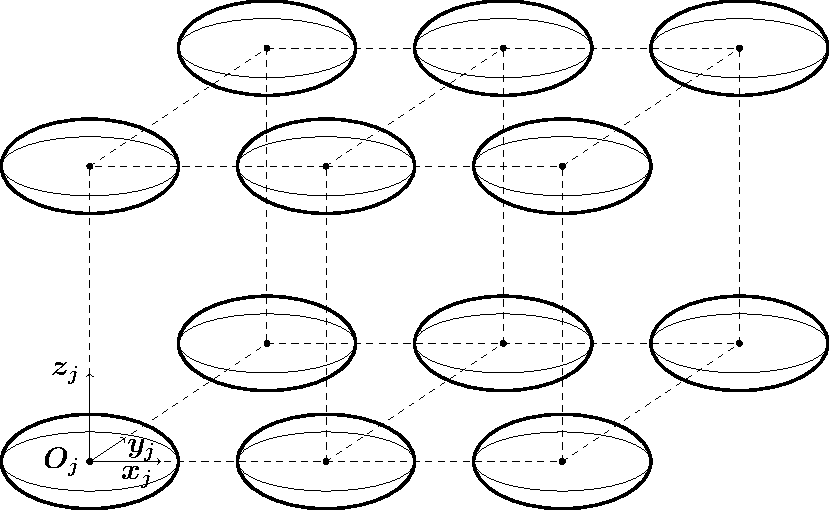
\includegraphics[width=12cm]{oblate-spheroids-periodic.pdf}
\caption{Периодическая система сжатых сфероидальных полостей в упругом пространстве}
\label{f:11:1b}
\end{figure}

С каждой точкой $O_j$ свяжем локальные декартовую $(x_j,y_j,z_j)$ и сонаправленную с ней сжатую сфероидальную системы координат $(\tilde\xi_j,\tilde\eta_j,\varphi_j)$. Считается, что декартовые системы координат с началами в точках $O_j$ сонаправлены.

Будем рассматривать задачу упругого деформирования пространства со сжатыми сфероидальными полостями $\Omega\backslash\bigg\{\bigcup\limits_{\alpha,\beta,\gamma}\omega_{\alpha\beta\gamma}\bigg\}$ под действием нагрузки, приложенной на бесконечности (одноосное, двуосное или всестороннее растяжение упругого пространства). Сфероидальные полости считаются свободными от нагрузки.

Соотношения между координатами можно описать формулами

\begin{equation*}
{x_i} = \tilde c\,\mathrm{ch}\tilde\xi_j\sin {\tilde\eta _i}\cos {\varphi _i},
\end{equation*}

\begin{equation}
{y_i} = \tilde c\,\mathrm{ch}\tilde\xi_j\sin {\tilde\eta _i}\sin {\varphi _i},
\label{eq:11:22k}
\end{equation}

\begin{equation*}
{z_i} = \tilde c\,\mathrm{sh}\tilde\xi_j\cos {\tilde\eta _i},
\end{equation*}

\begin{equation}
\left\{ {\begin{array}{*{20}{l}}
{{x_j} = {x_\alpha } + {x_{j\alpha }},}\\
{{y_j} = {y_\alpha } + {y_{j\alpha }},}\\
{{z_j} = {z_\alpha } + {z_{j\alpha }},}
\end{array}} \right.\qquad {\kern 1pt} j \ne \alpha ,\quad j,\alpha  = \overline {1,N},
\label{eq:11:23k}
\end{equation}

\noindent где $\overrightarrow {{O_j}{O_\alpha }}  = \left( {{x_{j\alpha }},{y_{j\alpha }},{z_{j\alpha }}} \right) = \left( {{r_{j\alpha }},{\theta _{j\alpha }},{\varphi _{j\alpha }}} \right)$.

Для определения НДС в рассматриваемом теле необходимо решить краевую задачу для уравнения Ламе относительно неизвестного вектора перемещения   $\mathbf{U}$ с граничными условиями

\begin{equation}
{\bf{FU}}{|_{{\Gamma _j}}} = 0
\end{equation}

\noindent и условиями на бесконечности одного из трех типов

\begin{equation}
{\bf{FU}}{|_{z =  \pm \infty }} =  \pm T{{\bf{e}}_z}\quad\text{(одноосное растяжение)},
\label{eq:11:1k}
\end{equation}

\begin{equation}
{\bf{FU}}{|_{\rho  = \infty }} = T{{\bf{e}}_\rho }\quad\text{(двуосное растяжение)},
\label{eq:11:2k}
\end{equation}

\begin{equation}
{\bf{FU}}{|_{r  = \infty }} = T{{\bf{e}}_r }\quad\text{(всестороннее растяжение)},
\label{eq:11:3k}
\end{equation}

\noindent где $\mathbf{FU}$~--- отвечающий перемещению $\mathbf{U}$ вектор усилий на соответствующей граничной поверхности; ${\Gamma _j} = \left\{ {\left( {{\tilde\xi_j},{\tilde\eta _j},{\varphi _j}} \right):\,{\tilde\xi_j} = {\tilde\xi_{0j}}} \right\}$.

Решение задачи будем искать в виде

\begin{equation}
{\bf{U}} = {\bf{\tilde U}} + {{\bf{U}}_0},
\end{equation}

\begin{equation}
{\bf{\tilde U}} = \sum\limits_{j = 1}^\infty {\sum\limits_{s = 1}^3 {\sum\limits_{n = 0}^\infty  {\sum\limits_{m=-n}^{n} {a_{s,n,m}^{(j)}} } } } {\bf{\tilde U}}_{s,n,m}^{ + (6)}\left( {{\tilde\xi_j},{\tilde\eta _j},{\varphi _j}} \right),
\label{eq:11:24k}
\end{equation}

\begin{equation}
{{\bf{U}}_0} = \frac{T}{{2G}}\left( { - \frac{\sigma }{{1 + \sigma }}{\rho}{{\bf{e}}_{{\rho}}} + \frac{1}{{1 + \sigma }}{z}{{\bf{e}}_z}} \right)\,\text{(одноосное растяжение)},
\label{eq:11:25k}
\end{equation}

\begin{equation}
{{\bf{U}}_0} = \frac{T}{{2G}}\left( {\frac{{1 - \sigma }}{{1 + \sigma }}{\rho}{{\bf{e}}_{{\rho}}} - \frac{{2\sigma }}{{1 + \sigma }}{z}{{\bf{e}}_z}} \right)\,\text{(двуосное растяжение)},
\label{eq:11:26k}
\end{equation}

\begin{equation}
{{\bf{U}}_0} = \frac{T}{2G}\frac{1-2\sigma}{1+\sigma}\left(\rho\mathbf{e}_\rho+z\mathbf{e}_z\right)\,\text{(всестороннее растяжение)},
\label{eq:11:27k}
\end{equation}

\noindent где $G$, $\sigma$~--- модуль сдвига и коэффициент Пуассона упругого пространства; $a_{s,n,m}^{(j)}$~--- неизвестные коэффициенты; перемещения $\mathbf{\tilde U}_{s,n,m}^{+(6)}$ приведены в формулах~\eqref{eq:1:89o}~--- \eqref{eq:1:94o}.

Относительно перемещения $\mathbf{\tilde U}$ граничные условия записывают следующим образом:

\begin{equation}
{\bf{F\tilde U}}{|_{{\Gamma _j}}} =  - {\bf{F}}{{\bf{U}}_0}{|_{{\Gamma _j}}};
\label{eq:11:28k}
\end{equation}

\begin{equation}
{\bf{F\tilde U}}{|_{z =  \pm \infty }} = 0\quad\text{(одноосное растяжение)};
\label{eq:11:29k}
\end{equation}

\begin{equation}
{\bf{F\tilde U}}{|_{\rho  = \infty }} = 0\quad\text{(двуосное растяжение)};
\label{eq:11:30k}
\end{equation}

\begin{equation}
{\bf{F\tilde U}}{|_{r  = \infty }} = 0\quad\text{(всестороннее растяжение)},
\label{eq:11:30ak}
\end{equation}

Вспомогательным перемещениям $\mathbf{U}_0$ отвечают следующие напряжения на поверхностях $\Gamma_j$ ($\mathbf{n}_j=\mathbf{e}_{\tilde\xi_j}$~--- вектор нормали на поверхности $\Gamma_j$):

\begin{equation}
{\bf{F}}{{\bf{U}}_0} = T\tilde H_j\,\mathrm{ch}\tilde\xi_j P_1(\cos\tilde\eta_j)\mathbf{e}_z\quad\text{(одноосное растяжение)};
\label{eq:11:k1}
\end{equation}

\begin{equation}
{\bf{F}}{{\bf{U}}_0} = -T\tilde H_j\,\mathrm{sh}\tilde\xi_j P_1^{(1)}(\cos\tilde\eta_j)\mathbf{e}_{\rho_j}\quad\text{(двуосное растяжение)};
\label{eq:11:k2}
\end{equation}

\begin{multline}
\mathbf{FU}_0=T\tilde H_j\bigg[-\mathrm{sh}\tilde\xi_j P_1^{(1)}(\cos\tilde\eta_j)\mathbf{e}_{\rho_j}+ \\
+\mathrm{ch}\tilde\xi_jP_1(\cos\tilde\eta_j)\mathbf{e}_z\bigg]\,\text{(всестороннее растяжение)}.
\label{eq:11:k3}
\end{multline}

Используя теоремы сложения~\eqref{eq:1:100o}, перемещение $\mathbf{\tilde U}$ можно записать полностью в системе координат с началом в точке $O_j$:

\begin{multline}
{\bf{\tilde U}} = \sum\limits_{s = 1}^3 {\sum\limits_{n = 0}^\infty  {\sum\limits_{m =  - n }^{n } {a_{s,n,m}^{(j)}} } } {\bf{\tilde U}}_{s,n,m}^{ +(6)}\left( {{\tilde\xi_j},{\tilde\eta _j},{\varphi _j}} \right) + \\
+ \sum\limits_{s=1}^3\sum\limits_{n = 0}^\infty\sum\limits_{m =  - n }^{n }{\bf{\tilde U}}_{s,n,m}^{ - (6)}\left( {{\tilde\xi_j},{\tilde\eta _j},{\varphi _j}} \right)\sum\limits_{\alpha  \ne j}\sum\limits_{t=1}^3\sum\limits_{k = 0}^\infty\mathop \sum \limits_{l =  - k}^{k}\tilde T_{t,k,l,\alpha}^{s,n,m,j}a_{t,k,l}^{(\alpha)}.
\label{eq:11:31k}
\end{multline}

В силу периодичности задачи вклад каждого слагаемого в формуле~\eqref{eq:11:24k} будет одинаковым, поэтому можно считать, что $a_{s,n,m}^{(j)}=a_{s,n,m}$.

После перехода в формуле~\eqref{eq:11:31k} к напряжениям и удовлетворения граничным условиям относительно неизвестных $a_{s,n,m}$ получаем бесконечную систему линейных алгебраических уравнений:

\begin{equation}
\sum\limits_{s=1}^3 a_{s,n,m}\tilde F_{s,n,m}^{+(k)}+\tilde F_{s,n,m}^{-(k)}\sum\limits_{t=1}^3\sum\limits_{k=0}^\infty\sum\limits_{l=-k}^k a_{t,k,l}\sum\limits_{\alpha\neq j}\tilde T_{t,k,l,\alpha}^{s,n,m,j}=F_{n,m}^{(k)};
\label{eq:11:32k}
\end{equation}
$$
n,m \in\mathbb{Z}:\quad n \ge 0,{\mkern 1mu} \quad {\kern 1pt} |m| \le n,\quad {\mkern 1mu} k =  - 1,{\mkern 1mu} {\kern 1pt} 0,{\mkern 1mu} {\kern 1pt} 1;\;\;\;{\mkern 1mu} {\kern 1pt} j = \overline {1,\infty},
$$

\noindent где $\tilde F_{s,n,m}^{\pm(k)}$~--- компоненты вектора напряжений на поверхности $\tilde\xi_j=\tilde\xi_{j0}$, отвечающего вектору перемещения $\tilde U_{s,n,m}^{\pm(6)}$:

$$
\mathbf{F\tilde U}_{s,n,m}^{\pm(6)}=\frac{\tilde H_j}{\tilde c}\bigg(\tilde F_{s,n,m}^{\pm(-1)}S_n^{m-1}\mathbf{e}_{-1}+\tilde F_{s,n,m}^{\pm(1)}S_n^{m+1}\mathbf{e}_1+\tilde F_{s,n,m}^{\pm(0)}S_n^m\mathbf{e}_0\bigg);
$$

\begin{equation*}
F_{n,m}^{(k)} =  -\frac{Td_2}{2G}{\delta _{n1}}{\delta _{m0}}{\delta _{k0}}\quad\text{(одноосное растяжение)},
\end{equation*}

\begin{equation*}
F_{n,m}^{(k)} =  -\frac{Td_1}{2G}{\delta _{n1}}{\delta _{m0\,}}(2{\delta _{k, - 1}} - {\delta _{k1}})\quad\text{(двуосное растяжение)},
\end{equation*}

\begin{equation*}
F_{n,m}^{(k)} =  -\frac{T}{2G}{\delta _{n1}}{\delta _{m0\,}}(\delta_{k0}d_2+2{\delta _{k, - 1}}d_1 - {\delta _{k1}}d_1)\quad\text{(всестороннее растяжение)}.
\end{equation*}

Явный вид компонент $\tilde F_{s,n,m}^{\pm(k)}$ не приводится ввиду их громоздкости. Они получаются из формул~\eqref{eq:1:89o}~--- \eqref{eq:1:99o}, \eqref{eq:10:25o}~--- \eqref{eq:10:27o}.

На рис.~\ref{f:11:35}~--- \ref{f:11:40} представлены нормальные напряжения на линии $AB$ в зависимости от расстояния между включениями при одноосном и двуосном растяжениях упругого пространства при $\sigma=0.38$, $d_1/d_2=0.5$.

При одноосном растяжении основной вклад в тензор напряжений вносят напряжения $\sigma_z/T$. Областью их концентрации являются границы полостей, и с приближением полостей друг к другу эти напряжения растут. Подобным свойством обладают напряжения $\sigma_x/T$ и $\sigma_y/T$.

При двуосном растяжении основной вклад в тензор напряжений вносят напряжения $\sigma_y/T$. Эти напряжения изменяются несущественно на отрезке $AB$ и с приближением полостей друг к другу возрастают. Напряжения $\sigma_z/T$ меняют знак на отрезке $AB$, оставаясь сжимающими вблизи его концов, и растягивающими~--- вблизи середины отрезка.

\begin{figure}[h!]
\centering\footnotesize
\parbox[b]{7.5cm}{\centering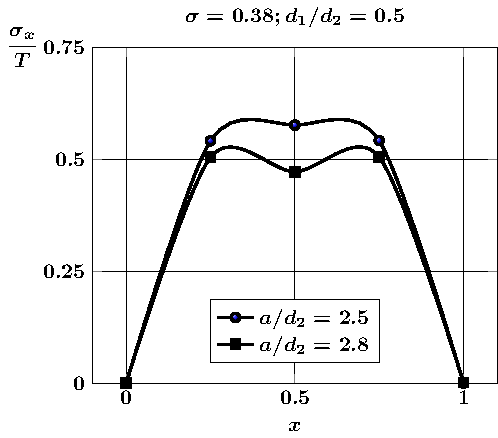
\includegraphics[width=7.8cm]{periodic-oblate-cav27-a-d50-t1-sig_x.pdf}
\caption{Напряжения $\sigma_x/T$ на линии $AB$ в зависимости от расстояния между полостями при одноосном растяжении
\label{f:11:35}}}\hfil\hfil
\parbox[b]{7.5cm}{\centering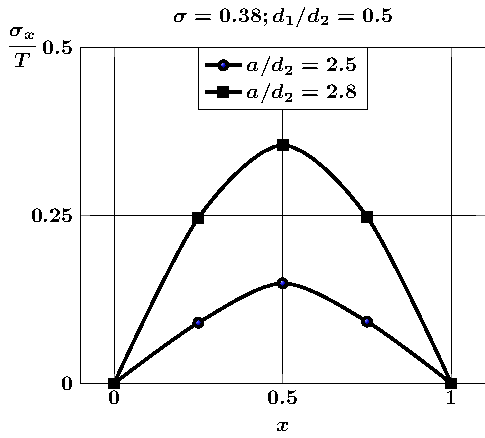
\includegraphics[width=7.6cm]{periodic-oblate-cav27-a-d50-t2-sig_x.pdf}
\caption{Напряжения $\sigma_x/T$ на линии $AB$ в зависимости от расстояния между полостями при двуосном растяжении
\label{f:11:36}}}
\end{figure}

\begin{figure}[h!]
\centering\footnotesize
\parbox[b]{7.5cm}{\centering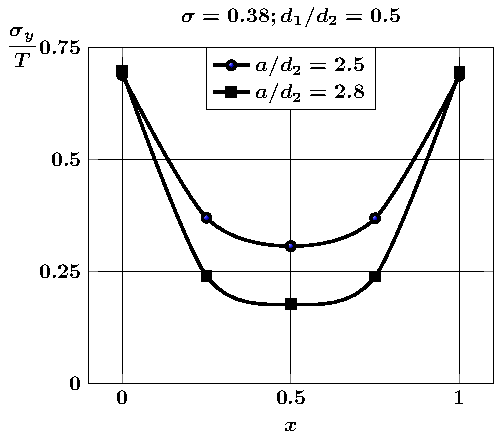
\includegraphics[width=7.6cm]{periodic-oblate-cav27-a-d50-t1-sig_y.pdf}
\caption{Напряжения $\sigma_y/T$ на линии $AB$ в зависимости от расстояния между полостями при одноосном растяжении
\label{f:11:37}}}\hfil\hfil
\parbox[b]{7.5cm}{\centering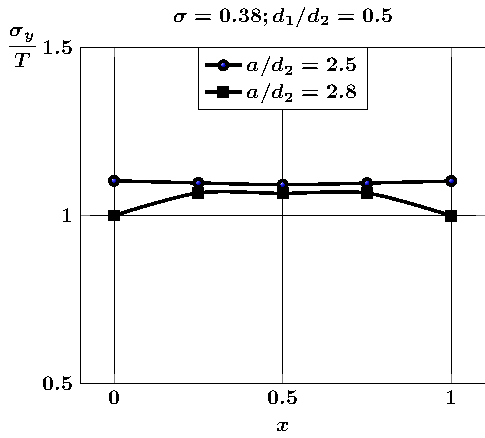
\includegraphics[width=7.6cm]{periodic-oblate-cav27-a-d50-t2-sig_y.pdf}
\caption{Напряжения $\sigma_y/T$ на линии $AB$ в зависимости от расстояния между полостями при двуосном растяжении
\label{f:11:38}}}
\end{figure}

\begin{figure}[h!]
\centering\footnotesize
\parbox[b]{7.5cm}{\centering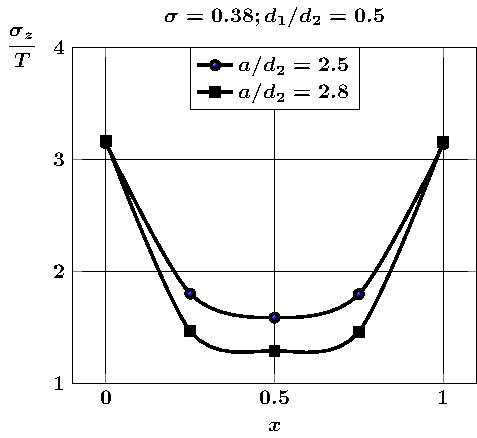
\includegraphics[width=7.6cm]{periodic-oblate-cav27-a-d50-t1-sig_z.pdf}
\caption{Напряжения $\sigma_z/T$ на линии $AB$ в зависимости от расстояния между полостями при одноосном растяжении
\label{f:11:39}}}\hfil\hfil
\parbox[b]{7.5cm}{\centering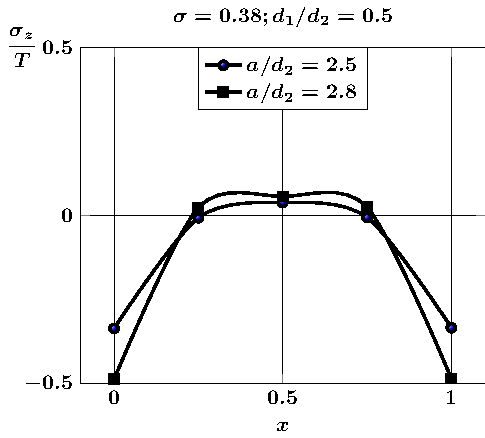
\includegraphics[width=7.8cm]{periodic-oblate-cav27-a-d50-t2-sig_z.pdf}
\caption{Напряжения $\sigma_z/T$ на линии $AB$ в зависимости от расстояния между полостями при двуосном растяжении
\label{f:11:40}}}
\end{figure}

\begin{figure}[h!]
\centering\footnotesize
\parbox[b]{7.5cm}{\centering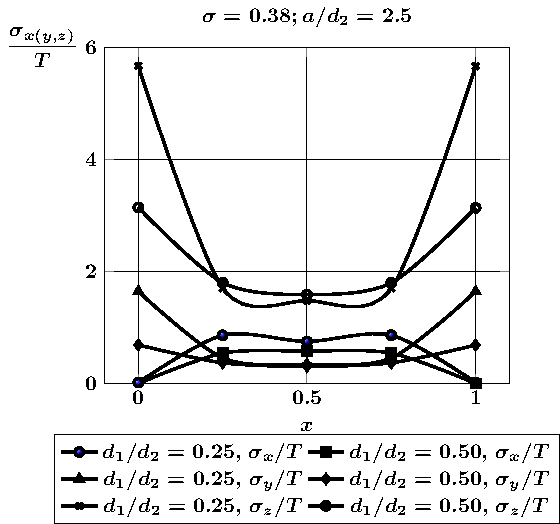
\includegraphics[width=7.8cm]{periodic-oblate-cav27-d-a25-t1.pdf}
\caption{Сравнение напряжений на линии $AB$ в зависимости от формы сфероидальной полости при одноосном растяжении
\label{f:11:41}}}\hfil\hfil
\parbox[b]{7.5cm}{\centering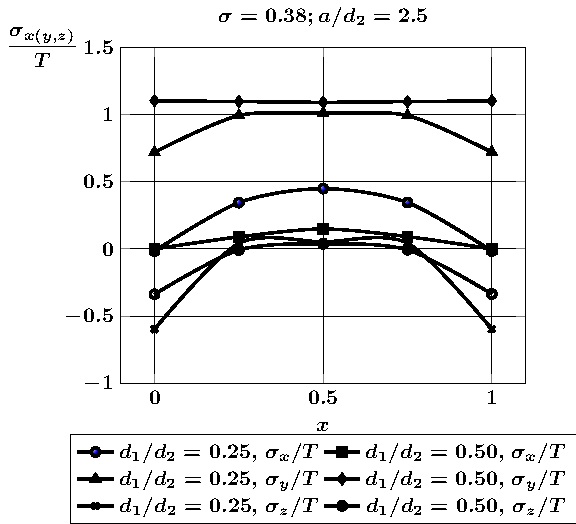
\includegraphics[width=8cm]{periodic-oblate-cav27-d-a25-t2.pdf}
\caption{Сравнение напряжений на линии $AB$ в зависимости от формы сфероидальной полости при двуосном растяжении
\label{f:11:42}}}
\end{figure}

На рис.~\ref{f:11:41}, \ref{f:11:42} представлено сравнение нормальных напряжений на линии $AB$ в зависимости от формы сжатой сфероидальной полости при одноосном и двуосном растяжениях упругого пространства при $a/d_2=2.5$. При одноосном растяжении в наибольшей степени зависят от формы полости напряжения $\sigma_z/T$ и $\sigma_y/T$, причем различия в значениях напряжений особенно заметны на границах полостей. С уменьшением отношения $d_1/d_2$ наблюдается резкая концентрация этих напряжений.

При двуосном растяжении зависимость от формы полости не столь существенна, как при одноосном растяжении. Уменьшение отношения $d_1/d_2$ не приводит к резкой концентрации напряжений.

\begin{table}[h!]
\centering
\caption{\centering Сравнение напряжений для разного количества полостей~периодической~структуры}
$
\begin{array}{|c|c|c|c|}
\hline
\text{Кол-во полостей} & \sigma_x/T & \sigma_y/T & \sigma_z/T \\
\hline
27 & 0.47211 & 0.17632 & 1.2920 \\
\hline
125 & 0.47208 & 0.17857 & 1.2947 \\
\hline
\end{array}
$
\label{t:11:3}
\end{table}

В табл.~\ref{t:11:3} приведено сравнение нормальных напряжений в средней точке отрезка $AB$ для разного количества (27 и 125) сжатых сфероидальных полостей периодической структуры при $a/d_2=2.8$, $d_1/d_2=0.5$ и при одноосном растяжении упругого пространства. Из таблицы видно, что увеличение числа полостей практически не меняет значения напряжений.


\section[Упругое пространство с периодической системой сжатых сфероидальных включений]{Упругое пространство с периодической системой сжатых сфероидальных включений\sectionmark{Упругое пространство с периодической системой сфероидальных включений}}\sectionmark{Упругое пространство с периодической системой сфероидальных включений}

Рассмотрим упругое пространство $\Omega$ и бесконечную систему сжатых сфероидальных включений $\{\omega_{\alpha\beta\gamma}\}_{\alpha,\beta,\gamma=-\infty}^\infty$, центры которых расположены в узлах $\{O_{\alpha\beta\gamma}\}_{\alpha,\beta,\gamma=-\infty}^\infty$ кубической периодической решетки со стороной $a$. Декартовыми координатами узлов решетки будут упорядоченные наборы чисел $\{(\alpha a,\beta a,\gamma a);\,\alpha,\beta,\gamma\in\mathbb{Z}\}$. Полуоси включений обозначим через $d_1$ и $d_2$ ($d_2>d_1$). Выполним линейное упорядочение узлов таким же образом, как в параграфе 6.1.\sloppy

В новой нумерации точка $O_{\alpha,\beta,\gamma}$ обозначается через $O_j$ (см.~рис.~\ref{f:11:1b}). С каждой точкой $O_j$ свяжем локальные декартовую $(x_j,y_j,z_j)$ и сонаправленную с ней сжатую сфероидальную системы координат $(\tilde\xi_j,\tilde\eta_j,\varphi_j)$. Считается, что декартовые системы координат с началами в точках $O_j$ сонаправлены.

Будем рассматривать задачу упругого деформирования пространства со сжатыми сфероидальными включениями под действием нагрузки, приложенной на бесконечности (одноосное, двуосное или всестороннее растяжения упругого пространства).

Соотношения между координатами можно описать формулами~\eqref{eq:11:22k}, \eqref{eq:11:23k}.

Предполагается, что упругие постоянные включений равны $(\sigma_j,G_j)$. Упругие постоянные матрицы будем считать равными $(\sigma,G)$.

Граничные условия в рассматриваемой задаче представляют собой условия сопряжения полей перемещений и напряжений на поверхностях $\Gamma_j$. Для того, чтобы их записать, представим вектор перемещений в упругом пространстве в виде

\begin{equation}
{\bf{U}} = \left\{ {\begin{array}{*{20}{l}}
{{\bf{\tilde U}}_j^ - ,\quad \left( {x,y,z} \right) \in \omega_j,}\\
{{{{\bf{\tilde U}}}^ + } + {{\bf{U}}_0},\quad \left( {x,y,z} \right) \in\Omega\backslash {\bigcup\limits_j\omega_j},}
\end{array}} \right.
\label{eq:11:23l}
\end{equation}

\noindent где $\omega_j = \left\{ {\left( {{\tilde\xi_j},{\tilde\eta _j},{\varphi _j}} \right):\, {\tilde\xi_j} < {\tilde\xi_{0j}}} \right\}$. Тогда условия сопряжения принимают следующий вид:

\begin{equation}
\left( {{{{\bf{\tilde U}}}^ + } + {{\bf{U}}_0}} \right){|_{{\Gamma _j}}} = {\bf{\tilde U}}_j^ - {|_{{\Gamma _j}}},
\label{eq:11:24l}
\end{equation}

\begin{equation}
\left( {{\bf{F\tilde U^+}} + {\bf{F}}{{\bf{U}}_0}} \right){|_{{\Gamma _j}}} = {\bf{F}}{{\bf{\tilde U^-}}_j}{|_{{\Gamma _j}}},\qquad {\kern 1pt} j = 1,{\mkern 1mu} {\kern 1pt} 2,\dots.
\label{eq:11:25l}
\end{equation}

\noindent Условия на бесконечности задаются формулами~\eqref{eq:11:1k}~--- \eqref{eq:11:3k}.

Решение задачи будем искать в виде

\begin{equation}
{\bf{\tilde U^+}} = \sum\limits_{j = 1}^\infty {\sum\limits_{s = 1}^3 {\sum\limits_{n = 0}^\infty  {\sum\limits_{m=-n}^{n} {a_{s,n,m}^{(j)}} } } } {\bf{\tilde U}}_{s,n,m}^{ + (6)}\left( {{\tilde\xi_j},{\tilde\eta _j},{\varphi _j}} \right),
\label{eq:11:26l}
\end{equation}

\begin{equation}
\mathbf{\tilde U}_j^- = {\sum\limits_{s = 1}^3 {\sum\limits_{n = 0}^\infty  {\sum\limits_{m=-n}^{n} {b_{s,n,m}^{(j)}} } } } {\bf{\tilde U}}_{s,n,m}^{ - (6)}\left( {{\tilde\xi_j},{\tilde\eta _j},{\varphi _j}} \right),
\label{eq:11:27l}
\end{equation}

\noindent где $G$, $\sigma$~--- модуль сдвига и коэффициент Пуассона упругого пространства; $a_{s,n,m}^{(j)}$, $b_{s,n,m}^{(j)}$~--- неизвестные коэффициенты; перемещения $\mathbf{\tilde U}_{s,n,m}^{\pm(6)}$ приведены в формулах~\eqref{eq:1:89o}~--- \eqref{eq:1:99o}.

Для представления вектора перемещений $\mathbf{\tilde U}^+$ в системах координат с началами $O_j$ можем использовать формулу~\eqref{eq:11:31k}.

В силу периодичности задачи вклад каждого слагаемого в формулах~\eqref{eq:11:26l}, \eqref{eq:11:27l} будет одинаковым, поэтому можно считать, что $a_{s,n,m}^{(j)}=\\=a_{s,n,m}$, $b_{s,n,m}^{(j)}=b_{s,n,m}$.

После перехода к напряжениям в формуле~\eqref{eq:11:31k} и удовлетворения условиям~\eqref{eq:11:24l}, \eqref{eq:11:25l} получаем бесконечную систему линейных алгебраических уравнений относительно неизвестных $a_{s,n,m}$, $b_{s,n,m}$:

\begin{multline}
\sum\limits_{s=1}^3 a_{s,n,m}\tilde E_{s,n,m}^{+(k)}(\sigma)+\tilde E_{s,n,m}^{-(k)}(\sigma)\sum\limits_{t=1}^3\sum\limits_{k=0}^\infty\sum\limits_{l=-k}^k a_{t,k,l}\sum\limits_{\alpha\neq j}\tilde T_{t,k,l,\alpha}^{s,n,m,j}= \\
=-E_{n,m}^{(k)}+\sum\limits_{s=1}^3 b_{s,n,m}\tilde E_{s,n,m}^{-(k)}(\sigma_j);
\label{eq:11:28l}
\end{multline}

\begin{multline}
\sum\limits_{s=1}^3 a_{s,n,m}\tilde F_{s,n,m}^{+(k)}(\sigma)+\tilde F_{s,n,m}^{-(k)}(\sigma)\sum\limits_{t=1}^3\sum\limits_{k=0}^\infty\sum\limits_{l=-k}^k a_{t,k,l}\sum\limits_{\alpha\neq j}\tilde T_{t,k,l,\alpha}^{s,n,m,j}= \\
=F_{n,m}^{(k)}+\frac{G_j}{G}\sum\limits_{s=1}^3 b_{s,n,m}\tilde F_{s,n,m}^{-(k)}(\sigma_j);
\label{eq:11:29l}
\end{multline}

\begin{equation}
n,m \in\mathbb{Z} :\quad n \ge 0,\quad |m| \le n,\quad k =  - 1,{\mkern 1mu} {\kern 1pt} 0,{\mkern 1mu} {\kern 1pt} 1,
\end{equation}

\noindent где $\tilde E_{s,n,m}^{\pm(k)}$~--- компоненты вектора перемещений $\mathbf{\tilde U}_{s,n,m}^{\pm(6)}$ на поверхности $\tilde\xi_j=\\=\tilde\xi_{0j}$; $\tilde F_{s,n,m}^{\pm(k)}$~--- компоненты вектора напряжений на поверхности $\tilde\xi_j=\tilde\xi_{0j}$, отвечающего вектору перемещения $\tilde U_{s,n,m}^{\pm(6)}$:
$$
\mathbf{\tilde U}_{s,n,m}^{\pm(6)}=\tilde E_{s,n,m}^{\pm(-1)}S_n^{m-1}\mathbf{e}_{-1}+\tilde E_{s,n,m}^{\pm(1)}S_n^{m+1}\mathbf{e}_1+\tilde E_{s,n,m}^{\pm(0)}S_n^m\mathbf{e}_0;
$$
$$
\mathbf{F\tilde U}_{s,n,m}^{\pm(6)}=\frac{\tilde H_j}{\tilde c}\bigg(\tilde F_{s,n,m}^{\pm(-1)}S_n^{m-1}\mathbf{e}_{-1}+\tilde F_{s,n,m}^{\pm(1)}S_n^{m+1}\mathbf{e}_1+\tilde F_{s,n,m}^{\pm(0)}S_n^m\mathbf{e}_0\bigg);
$$

\begin{equation*}
E_{n,m}^{(k)} =\frac{T\tilde c}{2G}\delta_{n1}\delta_{m0}\bigg[-\frac{2\sigma}{1+\sigma}\,\mathrm{ch}\tilde\xi_{0j}\delta_{k,-1}+\frac{\sigma}{1+\sigma}\,\mathrm{ch}\tilde\xi_{0j}\delta_{k1}+\frac{1}{1+\sigma}\,\mathrm{sh}\tilde\xi_{0j}\delta_{k0}\bigg],
\end{equation*}

\begin{equation*}
F_{n,m}^{(k)} =  -\frac{Td_2}{2G}{\delta _{n1}}{\delta _{m0}}{\delta _{k0}}\quad\text{(одноосное растяжение)};
\end{equation*}

\begin{equation*}
E_{n,m}^{(k)} =\frac{T\tilde c}{2G}\delta_{n1}\delta_{m0}\bigg[\frac{2-2\sigma}{1+\sigma}\,\mathrm{ch}\tilde\xi_{0j}\delta_{k,-1}-\frac{1-\sigma}{1+\sigma}\,\mathrm{ch}\tilde\xi_{0j}\delta_{k1}-\frac{2\sigma}{1+\sigma}\,\mathrm{sh}\tilde\xi_{0j}\delta_{k0}\bigg],
\end{equation*}

\begin{equation*}
F_{n,m}^{(k)} =  -\frac{Td_1}{2G}{\delta _{n1}}{\delta _{m0\,}}(2{\delta _{k, - 1}} - {\delta _{k1}})\quad\text{(двуосное растяжение)};
\end{equation*}

\begin{equation*}
E_{n,m}^{(k)} =\frac{T\tilde c}{2G}\delta_{n1}\delta_{m0}\frac{1-2\sigma}{1+\sigma}\bigg[2\,\mathrm{ch}\tilde\xi_{0j}\delta_{k,-1}-\mathrm{ch}\tilde\xi_{0j}\delta_{k1}+\mathrm{sh}
\tilde\xi_{0j}\delta_{k0}\bigg],
\end{equation*}

\begin{equation*}
F_{n,m}^{(k)} =  -\frac{T}{2G}{\delta _{n1}}{\delta _{m0\,}}(d_2\delta_{k0}+2d_1{\delta _{k, - 1}} - d_1{\delta _{k1}})\quad\text{(всестороннее растяжение)}.
\end{equation*}

\begin{figure}[h!]
\centering\footnotesize
\parbox[b]{7.5cm}{\centering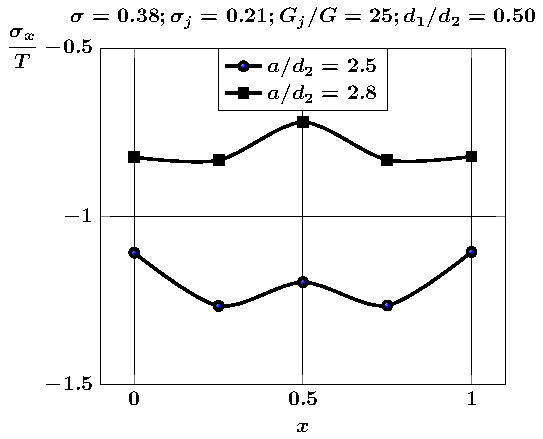
\includegraphics[width=8.1cm]{periodic-oblate-inc27-a-d50-g25-t1-sig_x.pdf}
\caption{Напряжения $\sigma_x/T$ на линии $AB$ в зависимости от расстояния между включениями при одноосном растяжении
\label{f:11:43}}}\hfil\hfil
\parbox[b]{7.5cm}{\centering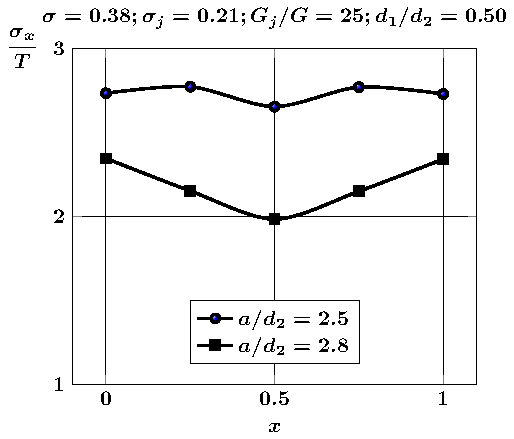
\includegraphics[width=7.6cm]{periodic-oblate-inc27-a-d50-g25-t2-sig_x.pdf}
\caption{Напряжения $\sigma_x/T$ на линии $AB$ в зависимости от расстояния между включениями при двуосном растяжении
\label{f:11:44}}}
\end{figure}

\begin{figure}[h!]
\centering\footnotesize
\parbox[b]{7.5cm}{\centering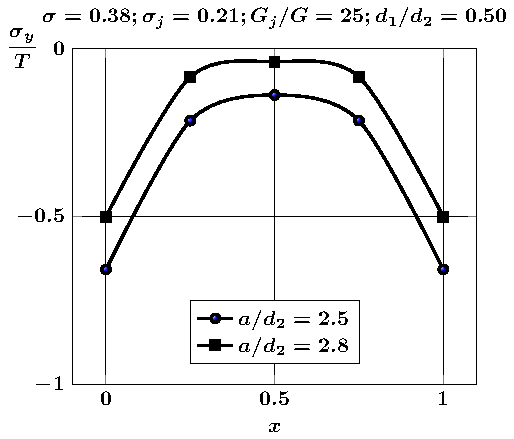
\includegraphics[width=7.8cm]{periodic-oblate-inc27-a-d50-g25-t1-sig_y.pdf}
\caption{Напряжения $\sigma_y/T$ на линии $AB$ в зависимости от расстояния между включениями при одноосном растяжении
\label{f:11:45}}}\hfil\hfil
\parbox[b]{7.5cm}{\centering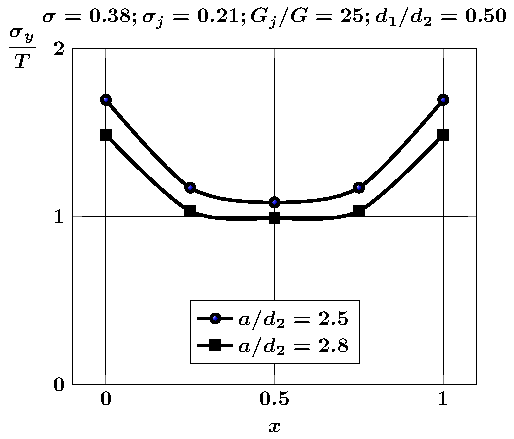
\includegraphics[width=7.8cm]{periodic-oblate-inc27-a-d50-g25-t2-sig_y.pdf}
\caption{Напряжения $\sigma_y/T$ на линии $AB$ в зависимости от расстояния между включениями при двуосном растяжении
\label{f:11:46}}}
\end{figure}

Явный вид компонент $\tilde E_{s,n,m}^{\pm(k)}$ и $\tilde F_{s,n,m}^{\pm(k)}$ не приводится ввиду их громоздкости. Они получаются из формул~\eqref{eq:1:73}~--- \eqref{eq:1:75}, \eqref{eq:1:89o}~--- \eqref{eq:1:99o}, \eqref{eq:10:25o}~--- \eqref{eq:10:27o}.

На рис.~\ref{f:11:43}~--- \ref{f:11:48} приведены нормальные напряжения на линии $AB$ в зависимости от расстояния между включениями при одноосном и двуосном растяжениях упругого пространства при $d_1/d_2=0.5$, $\sigma=0.38$, $\sigma_j=0.21$, $G_j/G=25$.
При одноосном растяжении основной вклад в тензор напряжений вносят напряжения $\sigma_x/T$ и $\sigma_z/T$. Напряжения $\sigma_x/T$ и $\sigma_y/T$ являются сжимающими на отрезке $AB$. Их модуль растет с приближением включений друг к другу. Напряжения $\sigma_z/T$ меняют знак на отрезке $AB$.

\begin{figure}[h!]
\centering\footnotesize
\parbox[b]{7.5cm}{\centering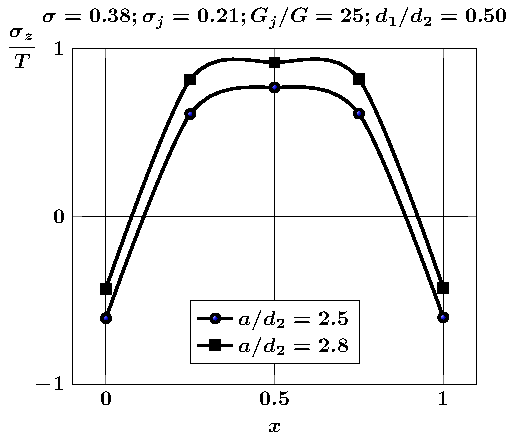
\includegraphics[width=7.8cm]{periodic-oblate-inc27-a-d50-g25-t1-sig_z.pdf}
\caption{Напряжения $\sigma_z/T$ на линии $AB$ в зависимости от расстояния между включениями при одноосном растяжении
\label{f:11:47}}}\hfil\hfil
\parbox[b]{7.5cm}{\centering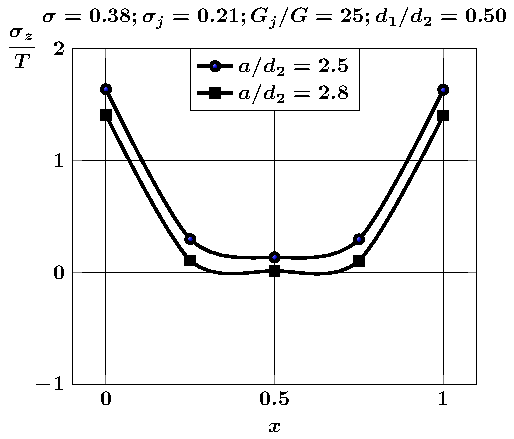
\includegraphics[width=7.8cm]{periodic-oblate-inc27-a-d50-g25-t2-sig_z.pdf}
\caption{Напряжения $\sigma_z/T$ на линии $AB$ в зависимости от расстояния между включениями при двуосном растяжении
\label{f:11:48}}}
\end{figure}

\begin{figure}[ht!]
\centering\footnotesize
\parbox[b]{7.5cm}{\centering\includegraphics[width=8cm]{oblate-inc27-8-a25-g25-t1.pdf}
\caption{Сравнение напряжения на линии $AB$ для периодической и тетрагональной структур при одноосном растяжении
\label{f:11:49}}}\hfil\hfil
\parbox[b]{7.5cm}{\centering\includegraphics[width=7.8cm]{oblate-inc27-8-a25-g25-t2.pdf}
\caption{Сравнение напряжения на линии $AB$ для периодической и тетрагональной структур при двуосном растяжении
\label{f:11:50}}}
\end{figure}

При двуосном растяжении основной вклад в тензор напряжений вносят напряжения $\sigma_x/T$, однако напряжения $\sigma_y/T$ и $\sigma_z/T$ являются значимыми. Для напряжений $\sigma_y/T$ и $\sigma_z/T$ область концентрации находится вблизи границы включений. При приближении включений друг к другу все напряжения возрастают.

На рис.~\ref{f:11:49}, \ref{f:11:50} представлено сравнение нормальных напряжений на линии $AB$ для периодической (27 включений) и тетрагональной (8 включений) структур при одноосном и двуосном растяжениях упругого пространства. Графики показывают, что напряжения $\sigma_y/T$ и $\sigma_z/T$ практически совпадают.

\end{russian}